\epigraphhead[650]{}
\part{规范场论}
\section*{规范对称性-内禀局域对称性}
我们考虑场的内禀局域变换，即变换参数依赖于时空位置：
\begin{equation}
	\psi(x)\rightarrow U(x)\psi(x) \tag{P.2.1}
\end{equation}
此时Lagrangian$\mathscr{L}_0$无法在此变换下保持不变,即表现为场沿某方向$n^\mu$的时空平移同时引起了内禀对称变换的变化，使得其导数$n^\mu\partial_\mu\psi$不为简单的几何表述。为了获得简单几何表述的导数形式，我们在变换的流形上定义平行移动：
\begin{equation}
	\Gamma(n)^y_x : \psi(x)\rightarrow\psi(y) \tag{P.2.2}
\end{equation}
即可将场从$x$点平行移动到$y$点。我们则可以定义其协变导数：
\begin{equation}
	n^\mu D_\mu\psi=\lim_{\epsilon\rightarrow 0}\frac{\psi(x+\epsilon n)-\Gamma(n)^{x+\epsilon n}_x\psi(x)}{\epsilon}\tag{P.2.3}
	\label{co-d}
\end{equation}
此时我们在Lagrangian中修改微分算符$\partial_\mu$为协变导数$D_\mu$，使得：
\begin{equation}
	D_\mu\Big( U(x)\psi(x)\Big)=U(x)\Big(D_\mu \psi(x)\Big)\tag{P.2.4}
\end{equation}
即表为协变导数同时具有变换：
\begin{equation}
	D_\mu\rightarrow U(x)D_\mu U^\dagger(x)\tag{P.2.5}
\end{equation}
此时修改后的Lagrangian动能项才能在局域变换下保持不变，即具有局域对称性：
\begin{equation}
	\mathscr{L}_0=\bar{\psi}(x)i\gamma^\mu D_\mu\psi(x)\tag{P.2.6}
\end{equation}
考虑在极小时空位移下的平行移动，我们可以将其展开为：
\begin{equation}
	\Gamma(n)^{x+\epsilon n}_x = 1 + i g\,\epsilon\, n^\mu A_\mu(x) +\mathcal{O}(\epsilon^2)\tag{P.2.7}
\end{equation}
其中$A_\mu$为平行移动的联络，而无量纲参数$g$则反映了平行移动的变化强度。代入\eqref{co-d}中，我们可得：
\begin{equation}
	D_\mu=\partial_\mu-ig A_\mu(x)\tag{P.2.8}
\end{equation}
其中引入的联络$A_\mu(x)$同时也是一个矢量场
而协变导数满足Jacobi恒等式：
\begin{equation}
	[D_\mu,[D_\nu,D_\rho]]+[D_\nu,[D_\rho,D_\mu]]+[D_\rho,[D_\mu,D_\nu]]=0\tag{P.2.9}
\end{equation}
对于协变导数，我们定义为局域对称性变换下的伴随表示，有：
\begin{align}
	D'_\mu&=\partial_\mu-ig A'_\mu(x)\notag\\
	&=U(x)D_\mu U^\dagger(x)=U(x)\Big(\partial_\mu-ig A_\mu(x)\Big)U^\dagger(x)\notag\\
	&=\partial_\mu+U(x)\Big(\partial_\mu U^\dagger(x)\Big)-igU(x)A_\mu(x)U^\dagger(x)\tag{P.2.10}
\end{align}
由此我们可知矢量场$A_\mu(x)$在局域对称变换下有如下变换形式：
\begin{equation}
	A_\mu(x)\rightarrow A'_\mu(x)=U(x)A_\mu(x)U^\dagger(x)+\frac{i}{g}U(x)\Big(\partial_\mu U^\dagger(x)\Big)\tag{P.2.11}
	\label{eq:gaugetr}
\end{equation}
由于矢量场本身允许具有内禀的规范对称性，场在规范空间中变换不改变最终描述的场本身。因此$A_\mu(x)$的变换可以看成其规范对称性变换，而我们也将$A_\mu(x)$称为规范场。

对于场强张量$F_{\mu\nu}$，可构建为规范群流形上的曲率张量，即：
\begin{equation}
	[D_\mu,D_\nu]=-ig F_{\mu\nu}\tag{P.2.12}
\end{equation}
则我们可得：
\begin{equation}
	F_{\mu\nu}(x)=\partial_\mu A_\nu(x)-\partial_\nu A_\mu(x)-ig[A_\mu(x),A_\nu(x)]\tag{P.2.13}
\end{equation}
场强$F_{\mu\nu}$具有反对称性，并且满足Bianchi恒等式：
\begin{equation}
	D_{\mu}F_{\nu\rho}+D_\nu F_{\rho\mu}+D_\rho F_{\mu\nu}=0\tag{P.2.14}
\end{equation}
我们还可以定义，场强$F_{\mu\nu}$的对偶：
\begin{equation}
\tilde{F}_{\mu\nu}=\frac{1}{2}\epsilon_{\mu\nu\rho\sigma}F^{\rho\sigma}\tag{P.2.15}
\end{equation}
我们可以将Bianchi恒等式写为：
\begin{equation}
D^\mu\tilde{F}_{\mu\nu}=0\tag{P.2.16}
\end{equation}
\chapter{量子电动力学-Abliean规范场理论}
\section{电磁相互作用与其费曼规则}
对于电磁场而言，$A_\mu$并不具有更高的内禀自由度，则参与电磁相互作用的费米子场将会具有内禀局域U(1)对称性，即：
\begin{equation}
	U(x)=e^{i\alpha(x)}
\end{equation}
而对应的耦合常数$g=-e$。此时协变导数为：
\begin{equation}
	D_\mu=\partial_\mu+ieA_\mu
\end{equation}
电磁场的规范变换则为：
\begin{equation}
	A_\mu\rightarrow A_\mu-\frac{1}{e}\partial_\mu\alpha(x)
\end{equation}
同样，此时电磁场$A_\mu$之间相互对易，即代表电磁场之间互不相干，我们又称电磁场为Abliean规范场。由此可得电磁场张量：
\begin{equation}
	F_{\mu\nu}=\partial_\mu A_\nu-\partial_\mu A_\nu
\end{equation}
则我们可得电磁场以及参与电磁相互作用的费米子场的总Lagrangian:
\begin{align}
	\mathscr{L}_{\text{QED}}&=\bar{\psi}(i\slashed{D}-m)\psi-\frac{1}{4}F_{\mu\nu}F^{\mu\nu}\notag\\
	&=i\bar{\psi}\slashed{\partial}\psi-m\bar{\psi}\psi-\frac{1}{4}F_{\mu\nu}F^{\mu\nu}-e\bar{\psi}\slashed{A}\psi
\end{align}
其中$e\bar{\psi}\slashed{A}\psi$即为费米子与电磁场的相互作用项。
以此我们可得运动方程：
\begin{align}
(i\slashed{\partial}-m)\psi=e \slashed{A}\psi\notag\\
\partial_\mu F^{\mu\nu}=e\bar{\psi}\gamma^\nu\psi
\end{align}
由此我们可得守恒流$J^\mu$，也即电流密度：
\begin{equation}
J^\mu=e\bar{\psi}\gamma^\mu\psi
\end{equation}

同时我们可构造广义动量：
\begin{equation}
\pi=\frac{\partial\mathscr{L}}{\partial\dot{\psi}}=i\psi^\dagger,\qquad\pi^\mu=\frac{\partial\mathscr{L}}{\partial\dot{A}_\mu}=F^{\mu0}-\eta^{\mu0}(\partial^\nu A_\nu)
\end{equation}
其中电磁场引用费曼规范，则我们可得哈密顿量：
\begin{equation}
\mathscr{H}=\bar{\psi}(-i\gamma^i\partial_i+m)\psi+\frac{1}{2}(\partial_i A_\mu\partial^i A^\mu-\dot{A}_\mu\dot{A}^\mu)+e\bar{\psi}\gamma^\mu\psi A_\mu
\end{equation}
而对于时空平移对称性的守恒流，即为能动张量：
\begin{equation}
T^{\mu\nu}=i\bar{\psi}\gamma^\mu\partial^\nu\psi-F^{\mu\rho}\partial^\nu A_\rho-(\partial^\rho A_\rho)\partial^\nu A^\mu-\eta^{\mu\nu}\mathscr{L}
\end{equation}
而QED的格林函数生成泛函则为：
\begin{equation}
Z[J^\mu,\bar{\eta},\eta]=\int\mathcal{D}A_\mu\mathcal{D}\bar{\psi}\mathcal{D}\psi\;e^{i\int\mathrm{d}x(\mathscr{L}_{\text{QED}}+A_\mu J^\mu+\bar{\psi}\eta+\bar{\eta}\psi)}
\end{equation}
在洛伦兹规范下 从运动方程中我们可以分别求解得带电费米子场和电磁场：
\begin{equation}
\psi(x)=\int\frac{\mathrm{d}\boldsymbol{p}}{(2\pi)^{3/2}\sqrt{2E(\boldsymbol{p})}}\sum^2_{r=1}\Big(b_r(\boldsymbol{p})u^r(\boldsymbol{p})e^{-ipk}+d^\dagger_r(\boldsymbol{p})v^r(\boldsymbol{p})e^{ikx}\Big)
\end{equation}
\begin{equation}
A_\mu(x)=\int\frac{\mathrm{d}\boldsymbol{k}}{(2\pi)^{3/2}\sqrt{2\omega(\boldsymbol{k})}}\sum^2_{r=1}\Big(\varepsilon^r_\mu(\boldsymbol{k}) a_r(\boldsymbol{k})e^{-ik}+\varepsilon^r_\mu(\boldsymbol{k})a^\dagger_r(\boldsymbol{k})e^{ikx}\Big)
\end{equation}

因此对于量子电动力学，我们可以根据场论的动力学理论计算出其费曼规则为：
\begin{itemize}
\item 传播子
\begin{figure}[H]
	\begin{minipage}{.5\textwidth}
		\centering
		\caption*{费米子传播子}
		\begin{equation*}
			\wick{\c1{\psi}(x_1)\c1{\bar{\psi}}(x_2)}=\frac{i}{\slashed{p}-m+i\epsilon}
		\end{equation*}
		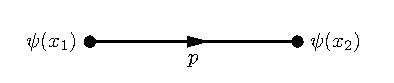
\includegraphics[width=.7\textwidth]{图/e-propa.pdf}
  %   \begin{fmffile}{e-propa}
  %             \begin{fmfgraph*}(100,40)
  %      \fmfleft{i}
  %      \fmfright{o}
  %      \fmflabel{$\psi(x_2)$}{o}
  %      \fmflabel{$\psi(x_1)$}{i}
  %      \fmfv{d.sh=circle,d.f=1,d.si=5pt}{i}
  %      \fmfv{d.sh=circle,d.f=1,d.si=5pt}{o}
  %      \fmf{fermion,tension=1,label=$k$}{i,o}
  %   \end{fmfgraph*}
  % \end{fmffile}
	\end{minipage}
	\begin{minipage}{.5\textwidth}
		\centering
				\caption*{光子传播子}
		\begin{equation*}
			\wick{\c1{A_\mu}(x_1)\c1{A_\nu}(x_2)}=\frac{-i\eta_{\mu\nu}}{k^2+i\epsilon}
		\end{equation*}
  % \begin{fmffile}{gam-propa}
  %             \begin{fmfgraph*}(100,40)
  %      \fmfleft{i}
  %      \fmfright{o}
  %      \fmflabel{$A_\nu(x_2)$}{o}
  %      \fmflabel{$A_\mu(x_1)$}{i}
  %      \fmfv{d.sh=circle,d.f=1,d.si=5pt}{i}
  %      \fmfv{d.sh=circle,d.f=1,d.si=5pt}{o}
  %      \fmf{boson,tension=1,label=$k$}{i,o}
  %   \end{fmfgraph*}
  % \end{fmffile}
		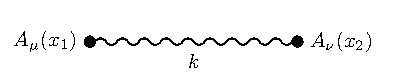
\includegraphics[width=.7\textwidth]{图/gam-propa.pdf}
	\end{minipage}
\end{figure}
\end{itemize}
\begin{itemize}
\item 顶点
\begin{figure}[H]
\begin{minipage}{.5\textwidth}
	\vspace{-20pt}
	\hspace{2cm}电磁相互作用顶点
\[\qquad\qquad\tilde{\Gamma}[A_\mu(x_1),\psi(x_2),\bar{\psi}(x_3)]\;=\;-ie\gamma^\mu\]
\end{minipage}
\begin{minipage}{.5\textwidth}
	\centering
%          \begin{fmffile}{qedint}
% \begin{fmfgraph*}(100,100)
%     \fmfleft{i1,i2}
%     \fmfright{i3}
%     \fmflabel{$\Bar{\psi} (x_3)$}{i2}
%     \fmflabel{$\psi (x_2)$}{i1}
%     \fmflabel{$A_\mu (x_1)$}{i3}
%     \fmf{fermion,label=$p$}{i1,v}
%     \fmf{fermion,label=$q$}{v,i2}
%     \fmf{boson,label=$k$}{v,i3}
%     \fmfv{d.sh=circle,d.f=1,d.si=5pt}{i1}
%     \fmfv{d.sh=circle,d.f=1,d.si=5pt}{i2}
%     \fmfv{d.sh=circle,d.f=1,d.si=5pt}{i3}
%   \end{fmfgraph*}
% \end{fmffile}
	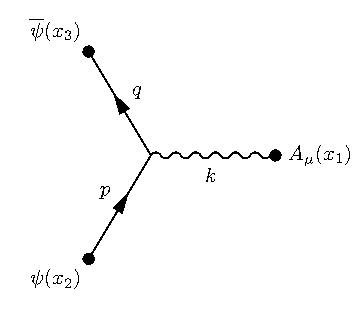
\includegraphics[width=.7\textwidth]{图/qedint.pdf}
\end{minipage}
\end{figure}
\item 外线
\subitem 入射费米子：\hspace{2cm}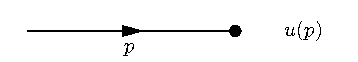
\includegraphics[scale=1]{图/in-e.pdf}%\hspace{1cm}\(u(\boldsymbol{p})\)
\vspace{5pt}
\subitem 出射费米子：\hspace{2cm}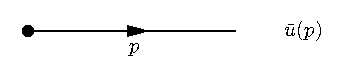
\includegraphics[scale=1]{图/out-e.pdf}%\hspace{1cm}\(\bar{u}(\boldsymbol{p})\)
\vspace{5pt}
\subitem 入射反费米子：\hspace{1.7cm}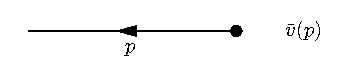
\includegraphics[scale=1]{图/in-pos.pdf}%\hspace{1cm}\(\bar{v}(\boldsymbol{p})\)
\vspace{5pt}
\subitem
出射反费米子：\hspace{1.7cm}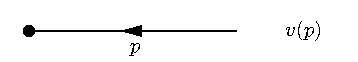
\includegraphics[scale=1]{图/out-pos.pdf}%\hspace{1cm}\(v(\boldsymbol{p})\)
\vspace{5pt}
\subitem 入射光子：\hspace{2.4cm}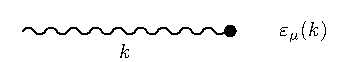
\includegraphics[scale=1]{图/in-gam.pdf}%\hspace{1cm}\(\varepsilon_\mu(\boldsymbol{k})\)
\vspace{5pt}
\subitem
出射光子：\hspace{2.4cm}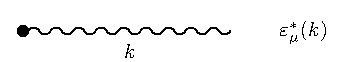
\includegraphics[scale=1]{图/out-gam.pdf}%\hspace{1cm}\(\varepsilon^*_\mu(\boldsymbol{k})\)
\end{itemize}
\section{Ward-高桥恒等式}
我们知道，对规范不变的QED系统来说，整个系统具有规范不变性，即各场在如下变换中保持运动方程不变：
\begin{equation}
	\begin{split}
		\delta A_\mu&=-\frac{1}{e}\partial_\mu\alpha(x)\\
		\delta \psi&=i\alpha(x)\psi\\
		\delta \bar{\psi}&=-i\alpha(x)\bar{\psi}
	\end{split}
\end{equation}
然而当我们考虑固定规范时，规范约束项则破坏了规范对称性。例如在$R_\xi$规范下，规范变换则会引起规范约束项产生额外的项。但是我们知道对于带电粒子的规范对称性而言，其不仅仅是一内禀的属性，更隐含了电荷守恒，因此在考虑电磁场与费米子场耦合时，不能简单的破坏掉规范对称性。

由此我们可以考虑有外源场情形下的QED，那么格林函数生成泛函则为：
\begin{equation}
	Z[J^\mu,\bar{\eta},\eta]=\int\mathcal{D}A_\mu\mathcal{D}\bar{\psi}\mathcal{D}\psi\exp\Big\{i\int\mathrm{d}x\Big(\bar{\psi}(i\slashed{D}-m)\psi-\frac{1}{4}F_{\mu\nu} F^{\mu\nu}-\frac{1}{2\xi}(\partial_\mu A^\mu)^2+A_\mu J^\mu+\bar{\psi}\eta+\bar{\eta}\psi\Big)\Big\}
\end{equation}
那么对于此时指数内的作用量，在规范变换下我们仍要保持其不变。不考虑前两项规范不变项，那么规范固定项及外源项在规范变换下产生的部分则需要为0，即：
\begin{equation}
	\int\mathrm{d}x\left[\frac{1}{\xi e}(\partial^\nu A_\nu)\partial^\mu\partial_\mu\alpha-\frac{1}{e}J^\mu\partial_\mu\alpha+i\alpha(\bar{\eta}\psi-\bar{\psi}\eta)\right]=0
\end{equation}
此时，我们需要考虑外源$J^\mu$在该系统下的表达形式，我们便可以考虑有效作用量。由\eqref{eq:effact}式，我们可得有效作用量：
\begin{equation}
	\Gamma[A_\mu,\psi,\bar{\psi}]=-i\ln Z[J^\mu,\bar{\eta},\eta]-\int\mathrm{d}x(A_\mu J^\mu+\bar{\eta}\psi+\bar{\psi}\eta)
\end{equation}
那么我们可得：
\begin{equation}
	\frac{\delta\Gamma}{\delta A_\mu}=-J^\mu,\qquad\frac{\delta\Gamma}{\delta\psi}=\bar{\eta},\qquad\frac{\delta\Gamma}{\delta\bar{\psi}}=-\eta
\end{equation}
那么将外源的表达式代入到对称性条件，即可的：
% \begin{small}
	\begin{equation}
		\int\mathrm{d}x\left[\frac{\delta\Gamma}{\delta A_\mu(x)}\partial_\mu\alpha(x)+\frac{\partial^\nu A_\nu(x)}{\xi }\partial^\mu\partial_\mu\alpha(x)+i\alpha(x)(\frac{\delta\Gamma}{\delta\psi(x)}\psi(x)+\bar{\psi}(x)\frac{\delta\Gamma}{\delta\bar{\psi(x)}})\right]=0
		\label{eq:wardori}
	\end{equation}
% \end{small}
这便是最原始形式的Ward-高桥恒等式。

由之前对有效作用量及外源场的讨论，有效作用量可表为：
\begin{multline}
	\Gamma=\int\mathrm{d}x\Big[\int\mathrm{d}y\Big(	\frac{1}{2}A_\mu(x)\bar{\Gamma}^{\mu\nu}_{A}(x,y)A_\nu(y)+\bar{\psi}(x)\bar{\Gamma}_{\psi}(x,y)\psi(y)\Big)	\\	+\int\mathrm{d}y\mathrm{d}z\;\bar{\psi}(x)A_\mu(y)\bar{\Gamma}^\mu_3(x,y,z)\psi(z)+\cdots\Big]
\end{multline}
我们易得有效作用量泛函导数：
\begin{align}
	\frac{\delta \Gamma}{\delta A_\mu(x)}&=\int\mathrm{d}y\; \bar{\Gamma}^{\mu\nu}_A(x,y)A_\nu(y)+\int\mathrm{d}y\mathrm{d}z\;\bar{\psi}(y)\bar{\Gamma}^\mu_3(x,y,z)\psi(z)+\cdots\\
	\frac{\delta \Gamma}{\delta \bar{\psi}(x)}&=\int\mathrm{d}y\;\bar{\Gamma}_\psi(x,y)\psi(y)+\int\mathrm{d}y\mathrm{d}z\;A_\mu(y)\bar{\Gamma}^\mu_3(x,y,z)\psi(z)+\cdots\\
	\frac{\delta \Gamma}{\delta {\psi}(x)}&=-\int\mathrm{d}y\;\bar{\psi}(y)\bar{\Gamma}_{\psi}(y,x)-\int\mathrm{d}y\mathrm{d}z\;\bar{\psi}(z)A_\mu(y)\bar{\Gamma}^\mu_3(z,y,x)+\cdots
\end{align}

若只考虑树图层面的Ward恒等式，将上式代入回\eqref{eq:wardori}式中，我们便发现包含费米子场的项与包含光子场的项实际线性独立。我们先考虑只包含光子场$A_\mu$的等式，即为：
\begin{equation}
	\int\mathrm{d}x\left[-\int\mathrm{d}y{D^{-1}}^{\mu\nu}(x-y)A_\nu(y) \partial_\mu\alpha(x)+\frac{\partial^\nu A_\nu(x)}{\xi}\partial^\mu\partial_\mu\alpha(x)\right]=0
\end{equation}
再对第二项中$\partial^\nu A_\nu$作分部积分，可得：
\begin{equation}
	\int\mathrm{d}x A_\nu(x)\Big[{D^{-1}}^{\mu\nu}\partial_\mu+\frac{1 }{\xi}\partial^\nu\partial_\mu\partial^\mu\Big]\alpha(x)=0
\end{equation}
作傅里叶变换，转移到动量空间，即可得：
\begin{equation}
	{D^{-1}}^{\mu\nu}k_\mu-\frac{1}{\xi}k^\nu k^2=0
\end{equation}
上式即为关于光子场的Ward-高桥恒等式。我们知道对于$R_\xi$规范下的光子传播子，有：
\begin{equation}
	D_{\mu\nu}=\frac{-i}{k^2}\left(\eta_{\mu\nu}-(1-\xi)\frac{k_\mu k_\nu}{k^2}\right),\qquad{D^{-1}}^{\mu\nu}=k^2\eta^{\mu\nu}+(\frac{1}{\xi}-1)k^\mu k^\nu
\end{equation}
完全满足Ward恒等式。而且此恒等式不仅仅对纯QED成立，还对多种相互作用共同参与的过程也成立。

而当我们取费曼规范$(\xi=1)$时，则有${D^{-1}}^{\mu\nu}k_\mu=0$。我们知道散射矩阵即为截腿格林函数，包含外线部分的传播子逆。因此对于一个有外线光子的过程，其散射振幅$\mathcal{M}=\varepsilon_\mu\mathcal{M}^\mu$，扣除掉对应外线光子的部分可得$\mathcal{M}^\mu$，即包含了对应光子的传播子逆，这样就有：
\begin{equation}
	k_\mu \mathcal{M}^\mu=0
\end{equation}

除此之外，我们可取$\frac{\delta\Gamma}{\delta A_\mu}$的次一级项以及$\frac{\delta\Gamma}{\delta\psi}$的首阶项，即可得出只包含费米子场的等式：
\begin{multline}
	\int\mathrm{d}x\Big[\int\mathrm{d}y\mathrm{d}z\,\bar{\psi}(y)\bar{\Gamma}^\mu_3(x,y,z)\psi(z)\partial_\mu\alpha(x)\\+i\alpha(x)\Big(\int\mathrm{d}z\bar{\psi}(x)\bar{\Gamma}_\psi(x,z)\psi(z)-\int\mathrm{d}y\bar{\psi}(y)\bar{\Gamma}_\psi(y,x)\psi(x)\Big)\Big]=0
\end{multline}
考虑树图层面的传播子，有$\bar{\Gamma}_\psi(x,y)=S^{-1}(x-y)$。对于第一项，我们对变量$x$作分部积分，化为对3点函数的导数形式，然后我们将上式后两项中的$x$变量用$\delta$函数替换为变量$y,z$，便可使整个等式两边夹同样的费米子场，并同时对三个变量积分，即可得：
\begin{equation}
	\bar{\psi}(y)\Big[i\frac{\partial}{\partial x^\mu}\bar{\Gamma}^\mu_3(x,y,z)+S^{-1}(y-z)\delta(x-y)-S^{-1}(y-z)\delta(x-z)\Big]\psi(z)=0
\end{equation}
则考虑动量空间，$x,y,z$三点分别依次对应光子动量$k$，费米子动量$q$和反费米子动量$p$（方向皆为入射顶点方向），可得：
\begin{equation}
	(2\pi)^4\delta(k+q+p)\Big(k_\mu\tilde{\Gamma}^\mu(k,q,p)+S^{-1}(p)-S^{-1}(-q)\Big)=0
\end{equation}
最终我们可得关于费米子场的Ward-高桥恒等式：
\begin{equation}
	k_\mu\tilde{\Gamma}^\mu(k,q,p)=S^{-1}(-q)-S^{-1}(p)
	\label{eq:wardf}
\end{equation}

若考虑树图层面的3点顶点函数，则$\tilde{\Gamma}^\mu(k,q,p)=\gamma^\mu$，代入传播子逆，即为：
\begin{equation}
\slashed{k}=-\slashed{q}-\slashed{p}
\end{equation}
恰好为动量守恒等式。
\section{QED散射过程}
\subsection*{非极化散射过程}
最简单基本的QED相互作用散射过程，便是正负电子对湮灭以及正负$\mu$子对产生：
\begin{equation}
e^- +e^+\longrightarrow \mu^- +\mu^+
\end{equation}
这样的一个散射的首阶相互作用过程有且仅有一个树图级别的费曼图来描述
\begin{center}
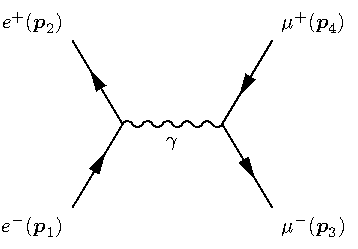
\includegraphics[width=.35\linewidth]{图/eemm.pdf}
%  \begin{fmffile}{eemumu}
%   \fmfframe(20,20)(20,20){\begin{fmfgraph*}(120,80)
%     \fmfleft{i1,i2}
%     \fmfright{o1,o2}
%     \fmflabel{$e^-(\boldsymbol{p}_1)$}{i1}
%     \fmflabel{$e^+(\boldsymbol{p}_2)$}{i2}
%     \fmflabel{$\mu^-(\boldsymbol{p}_3)$}{o1}
%     \fmflabel{$\mu^+(\boldsymbol{p}_4)$}{o2}
%     \fmf{fermion}{i1,v1}
%     \fmf{fermion}{v1,i2}
%     \fmf{fermion}{o2,v2}
%     \fmf{fermion}{v2,o1}
%     \fmf{boson,label=\(\gamma\)}{v1,v2}
%   \end{fmfgraph*}}
% \end{fmffile}
\end{center}
那么根据图中的动量以及费曼规则，我们可以得出其散射振幅：
\begin{equation}
-i\mathcal{M}=\bar{v}({p}_2)(-ie\gamma^\mu)u({p}_1)\frac{-i\eta_{\mu\nu}}{(p_1+p_2)^2}\bar{u}({p}_3)(-ie\gamma^\nu)v({p}_4)
\end{equation}
则我们可易得振幅的模方为：
% \begin{small}
	\begin{equation}
|\mathcal{M}|^2=\frac{e^4\eta_{\mu\nu}\eta_{\lambda\rho}}{(p_1+p_2)^4}\Big(\bar{u}(p_1)\gamma^\rho v(p_2)\Big)\Big(\bar{v}(p_2)\gamma^\mu u(p_1)\Big)\Big(\bar{u}(p_3)\gamma^\nu v(p_4)\Big)\Big(\bar{v}(p_4)\gamma^\lambda u(p_3)\Big)
\end{equation}
% \end{small}
那么当我们进一步计算散射过程可观测量时，则需要考虑极化的因素。对于非极化的散射过程，初态即为非极化粒子束，那么我们则需要对初态粒子的自旋求平均值。而对于末态，则粒子的可以为任意的极化状态，那么我们则要考虑所有可能的末态自旋，即对末态自旋求和。

对于非极化的初态电子，每个电子有2个自旋态，那么自旋态求平均则有一个$\frac{1}{4}$的因子。而对于费米子的自旋求和，则为对其螺旋度求和，即$\gamma^\mu$矩阵4分量求迹。那么最终我们对电子和$\mu$子分别进行自旋求和，然后再乘上初态平均的因子，且利用\eqref{eq:helsum}式的结果，我们可得：
\begin{equation}
\frac{1}{4}\sum_{\text{spin}}|\mathcal{M}|^2=\frac{e^4\eta_{\mu\nu}\eta_{\lambda\rho}}{4(p_1+p_2)^4}\mathrm{tr}\Big[(\slashed{p}_1+m_e)\gamma^\rho(\slashed{p}_2-m_e)\gamma^\mu\Big]\mathrm{tr}\Big[(\slashed{p}_3+m_\mu)\gamma^\nu(\slashed{p}_4-m_\mu)\gamma^\lambda\Big]
\end{equation}
由附录中\eqref{eq:gmtr}式，我们可得：
% \begin{small}
\begin{equation}
\overline{|\mathcal{M}|}^2=8e^4\frac{(p_1\cdot p_4)(p_2\cdot p_3)+(p_1\cdot p_3)(p_2\cdot p_4)+m_e^2(p_3\cdot p_4)+m_\mu^2(p_1\cdot p_2)+2m_e^2 m_\mu^2}{(p_1+p_2)^4}
\end{equation}
% \end{small}
利用四动量守恒及在壳条件，且由\eqref{eq:madsum}式，可将振幅模方化简为：
\begin{equation}
\begin{split}
\overline{|\mathcal{M}|}^2&=8e^4\frac{(p_1\cdot p_4)^2+(p_1\cdot p_3)^2+(m_e^2+m_\mu^2)(m_e^2+p_1\cdot p_2)}{(2p_1\cdot p_2+2m_e^2)^2}\\
&=8e^4\frac{(p_1\cdot p_3)^2+(\frac{s}{2}-p_1\cdot p_3)^2+\frac{s}{2}(m_e^2+m_\mu^2)}{s^2}
\end{split}
\end{equation}
%在通常的高能物理能区，电子的质量极其地微小

对于高能标下的该散射过程，由于电子质量和$\mu$子质量都非常小，所以可以忽略不记\(m_e\approx m_\mu\approx0\)。并且将所有四动量内积项转换为用Mandelstam表示的形式
%\footnote{粒子质量可忽略，且可考虑在质心系\[\begin{split}s&\approx2p_1\cdot p_2\approx2p_3\cdot p_4\\t&\approx-2p_1\cdot p_3\approx -2p_2\cdot p_4\\u&\approx-2p_1\cdot p_4\approx -2p_2\cdot p_3	\end{split}\]}
，那么结果可以写为：
\begin{equation}
\overline{|\mathcal{M}|}^2\approx2e^4\frac{u^2+t^2}{s^2}=2e^4\left(1+2\frac{t}{s}+2\frac{t^2}{s^2}\right)
\end{equation}
由于这一类过程的振幅模方反比于$s^2$，我们通常称之为$s$反应道。

此时我们已经可以计算具体的可观测量，即散射截面。由\eqref{eq:difxsec}式，我们可得二体散射的微分截面：
\begin{equation}
\begin{split}
\frac{\mathrm{d}\sigma}{\mathrm{d}\Omega}=\frac{\overline{|\mathcal{M}|}^2}{64\pi^2 s}\sqrt{\frac{1-\frac{4m_\mu^2}{s}}{1-\frac{4m_e^2}{s}}}
\end{split}
\end{equation}
其中$\alpha=\frac{e^2}{4\pi}$为精细结构常数。代入振幅模方可得：
\begin{equation}
\begin{split}
\frac{\mathrm{d}\sigma}{\mathrm{d}\Omega}&=\frac{\alpha^2}{2s}\left(1+2\frac{t}{s}+2\frac{t^2}{s^2}-4(m_e^2+m_\mu^2)(1+\frac{t}{s})+2(m_e^2+m_\mu^2)^2\right)\sqrt{\frac{s-{4m_\mu^2}}{s-{4m_e^2}}}\\&\approx\frac{\alpha^2}{2s}\left(1+2\frac{t}{s}+2\frac{t^2}{s^2}\right)
\end{split}
\end{equation}

考虑选取质心系作为我们的参考系，那么$\boldsymbol{p}_1$和$\boldsymbol{p}_2$等大反向，而$\boldsymbol{p}_1$和$\boldsymbol{p}_3$之间的夹角则为横向的散射角$\theta$。由于Mandelstam变量具有洛伦兹不变性，因此这三个变量在我们选取特定参考系时都不会发生改变。此时我们可计算出：
\begin{equation}
p_1\cdot p_3=\frac{s}{4}\left(1-\sqrt{(1-\frac{4m_\mu^2}{s})(1-\frac{4m_e^2}{s})}\cos\theta\right)=\frac{m_e^2+m_\mu^2-t}{2}
\end{equation}
而在极端相对论情形质心系中，则有Mandelstam变量和横向散射角$\theta$的关系：
\begin{equation}
t\approx-\frac{s}{2}(1-\cos\theta),\qquad u\approx-\frac{s}{2}(1+\cos\theta)
\end{equation}
微分截面则可表示为径向角$\theta$的函数：
\begin{equation}
\begin{split}
\frac{\mathrm{d}\sigma}{\mathrm{d}\Omega}(\theta)&=\frac{\alpha^2}{4s}\left(1+(1-\frac{4m_\mu^2}{s})(1-\frac{4m_e^2}{s})\cos^2\theta+\frac{4(m_e^2+m_\mu^2)}{s}\right)\sqrt{\frac{s-4m_\mu^2}{s-4m_e^2}}\\
&\approx\frac{\alpha^2}{4s}(1+\cos^2\theta)
\end{split}
\end{equation}
那么对立体角进行积分，我们则可得该过程的总散射截面为：
\begin{equation}
\sigma=\frac{4\pi\alpha^2}{3s}\left(1+\frac{2}{s}(m_e^2+m_\mu^2)+\frac{4}{s^2}m_e^2 m_\mu^2\right)\sqrt{\frac{s-4m_\mu^2}{s-4m_e^2}}\approx\frac{4\pi\alpha^2}{3 s}
\end{equation}

\begin{itemize}
\item 另外考虑电子和$\mu$子的外围散射过程：
\end{itemize}
\begin{equation}
e^- +\mu^-\longrightarrow e^-+\mu^-
\end{equation}
该过程的树图级别费曼图为：
% \newline
\begin{figure}[h]
\centering
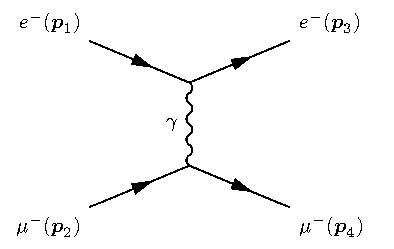
\includegraphics[width=0.33\textwidth]{图/emem.pdf}
% \begin{fmffile}{emu_emu}
%   \begin{fmfgraph*}(120,80)
%     \fmfleft{i1,i2}
%     \fmfright{o1,o2}
%     \fmflabel{$\mu^-(\boldsymbol{p}_2)$}{i1}
%     \fmflabel{$e^-(\boldsymbol{p}_1)$}{i2}
%     \fmflabel{$\mu^-(\boldsymbol{p}_3)$}{o1}
%     \fmflabel{$e^-(\boldsymbol{p}_4)$}{o2}
%     \fmf{fermion}{i1,v1,o1}
%     \fmf{fermion}{i2,v2,o2}
%     \fmf{photon,label=$\gamma$}{v1,v2}
%   \end{fmfgraph*}
% \end{fmffile}
\caption{}
\end{figure}
% \newline
则我们可得散射振幅为：
\begin{equation}
-i\mathcal{M}=\bar{u}({p}_3)(-ie\gamma^\mu)u({p}_1)\frac{-i\eta_{\mu\nu}}{(p_1-p_3)^2}\bar{u}({p}_4)(-ie\gamma^\nu)u({p}_2)
\end{equation}
则同理，并且我们考虑高能情形下的极端相对论极限，我们可计算的振幅模方为：
\begin{equation}
\overline{|\mathcal{M}|}^2\approx8e^4\frac{(p_1\cdot p_2)(p_3\cdot p_4)+(p_1\cdot p_4)(p_2\cdot p_3)}{(p_1-p_3)^2}\approx2e^4\frac{s^2+u^2}{t^2}
\end{equation}
我们通常将这种过程称为$t$反应道。

我们可得微分截面：
\begin{equation}
\frac{\mathrm{d}\sigma}{\mathrm{d}\Omega}(\theta)\approx\frac{\alpha^2}{2s}\frac{4+(1+\cos\theta)^2}{(1-\cos\theta)^2}
\end{equation}
我们可看到，这样的过程在$0\textdegree$角处极大地增幅。

\subparagraph{Bhabha散射}即为正负电子之间发生对撞，之后仍然产生一对正负电子的过程：
\begin{equation}
e^-+e^+\longrightarrow\; e^-+e^+
\end{equation}
对于这样的一个相互作用过程，我们可以用两个不同的费曼图来描述，分别对应$s$反应道和$t$反应道。由量子力学的相干叠加原理，实际的过程则是这两个反应道相干叠加的结果。
\begin{figure}[h]
\centering
	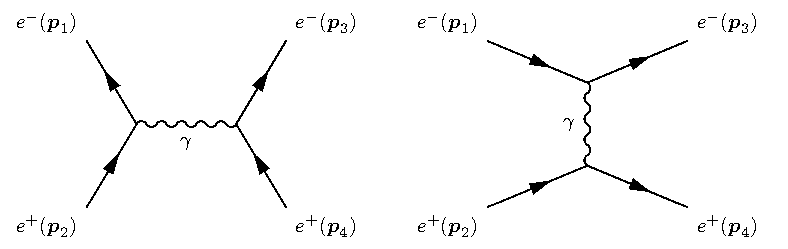
\includegraphics[width=.75\textwidth]{图/bhabha.pdf}
 % \vspace{20pt}
%  \begin{fmffile}{bhabha_s}
%   \begin{fmfgraph*}(120,80)
%     \fmfleft{i1,i2}
%     \fmfright{o1,o2}
%     \fmflabel{$e^-(\boldsymbol{p}_2)$}{i1}
%     \fmflabel{$e^-(\boldsymbol{p}_1)$}{i2}
%     \fmflabel{$e^-(\boldsymbol{p}_4)$}{o1}
%     \fmflabel{$e^-(\boldsymbol{p}_3)$}{o2}
%     \fmf{fermion}{i1,v1,i2}
%     \fmf{fermion}{o1,v2,o2}
%     \fmf{photon,label=$\gamma$}{v1,v2}
%   \end{fmfgraph*}
% \end{fmffile} \qquad\qquad \begin{fmffile}{bhabha_t}
%   \begin{fmfgraph*}(120,80)
%     \fmfleft{i1,i2}
%     \fmfright{o1,o2}
%     \fmflabel{$e^-(\boldsymbol{p}_2)$}{i1}
%     \fmflabel{$e^-(\boldsymbol{p}_1)$}{i2}
%     \fmflabel{$e^-(\boldsymbol{p}_4)$}{o1}
%     \fmflabel{$e^-(\boldsymbol{p}_3)$}{o2}
%     \fmf{fermion}{i1,v1,o1}
%     \fmf{fermion}{i2,v2,o2}
%     \fmf{photon,label=$\gamma$}{v1,v2}
%   \end{fmfgraph*}
% \end{fmffile}
 % \vspace{20pt}
 \caption{}
\end{figure}
根据费曼图我们可以得到具体的散射振幅，而总的散射振幅则为这两张费曼图对应的散射振幅之和：
\begin{equation}
\begin{split}
-i\mathcal{M}=&\bar{v}({p}_2)(-ie\gamma^\mu)u({p}_1)\frac{-i\eta_{\mu\nu}}{(p_1+p_2)^2}\bar{u}({p}_3)(-ie\gamma^\nu)v({p}_4)\\&+\bar{u}({p}_3)(-ie\gamma^\mu)u({p}_1)\frac{-i\eta_{\mu\nu}}{(p_1-p_3)^2}\bar{v}({p}_2)(ie\gamma^\nu)v({p}_4)
\end{split}
\end{equation}
那么振幅模方则是该散射振幅之和的模方，同样考虑极端相对论情形：
\begin{equation}
\overline{|\mathcal{M}|}^2=2e^4\left(\frac{u^2+t^2}{s^2}+\frac{s^2+u^2}{t^2}+\frac{2u^2}{s\cdot t}\right)
\end{equation}
微分截面为：
\begin{equation}
\frac{\mathrm{d}\sigma}{\mathrm{d}\Omega}(\theta)=\frac{\alpha^2}{2s}\left(\frac{1+\cos^2\theta}{2}+\frac{4+\cos\theta(1+\cos\theta)^2}{(1-\cos\theta)^2}\right)
\end{equation}


\subparagraph{M\o{}ller散射}即为电子和电子之间的散射：
\begin{equation}
e^-+e^-\longrightarrow\; e^-+e^-
\end{equation}
\begin{figure}[h]
\centering
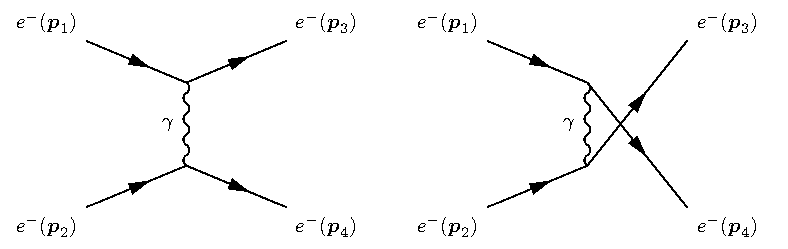
\includegraphics[width=0.75\textwidth]{图/moeller.pdf}
%  \vspace{20pt}
%  \begin{fmffile}{moeller_t}
%   \begin{fmfgraph*}(120,80)
%     \fmfleft{i1,i2}
%     \fmfright{o1,o2}
%     \fmflabel{$e^-(\boldsymbol{p}_2)$}{i1}
%     \fmflabel{$e^-(\boldsymbol{p}_1)$}{i2}
%     \fmflabel{$e^-(\boldsymbol{p}_4)$}{o1}
%     \fmflabel{$e^-(\boldsymbol{p}_3)$}{o2}
%     \fmf{fermion}{i1,v1,o1}
%     \fmf{fermion}{i2,v2,o2}
%     \fmf{photon,label=$\gamma$}{v1,v2}
%   \end{fmfgraph*}
% \end{fmffile} \qquad\qquad\qquad\begin{fmffile}{moeller_u}
%   \begin{fmfgraph*}(120,80)
%     \fmfleft{i1,i2}
%     \fmfright{o1,o2}
%     \fmflabel{$e^-(\boldsymbol{p}_2)$}{i1}
%     \fmflabel{$e^-(\boldsymbol{p}_1)$}{i2}
%     \fmflabel{$e^-(\boldsymbol{p}_4)$}{o1}
%     \fmflabel{$e^-(\boldsymbol{p}_3)$}{o2}
%     \fmf{fermion}{i1,v1}
%     \fmf{fermion}{i2,v2}
%     \fmf{phantom}{v1,o1}
%     \fmf{phantom}{v2,o2}
%     \fmf{fermion,tension=0}{v1,o2}
%     \fmf{fermion,tension=0}{v2,o1}
%     \fmf{photon,label=$\gamma$}{v1,v2}
%   \end{fmfgraph*}
% \end{fmffile}
%  \vspace{20pt}
\caption{}
\end{figure}
我们知道，如果$t$反应道的末态粒子为全同粒子，那么这两粒子则具有交换对称性不可分辨。因此则会有右图费曼图，即产生一个额外的反应道。这一个额外的反应道我们称之为$u$反应道。

对于这个散射过程，我们可以得到其散射振幅：
\begin{equation}
\begin{split}
-i\mathcal{M}=&\bar{u}({p}_3)(-ie\gamma^\mu)u({p}_1)\frac{-i\eta_{\mu\nu}}{(p_1-p_3)^2}\bar{u}({p}_4)(-ie\gamma^\nu)u({p}_2)\\
&+\bar{u}({p}_4)(-ie\gamma^\mu)u({p}_1)\frac{-i\eta_{\mu\nu}}{(p_1-p_4)^2}\bar{u}({p}_3)(-ie\gamma^\nu)u({p}_2)
\end{split}
\end{equation}

在极端相对论情形下，振幅模方为：
\begin{equation}
\overline{|\mathcal{M}|}^2=2e^4\left(\frac{s^2+u^2}{t^2}+\frac{s^2+t^2}{u^2}+\frac{2s^2}{t\cdot u}\right)
\end{equation}
微分截面为：
\begin{equation}
\frac{\mathrm{d}\sigma}{\mathrm{d}\Omega}(\theta)=\frac{\alpha^2}{2s}\left(\frac{4+(1+\cos\theta)^2}{(1-\cos\theta)^2}+\frac{4+(1-\cos\theta)^2}{(1+\cos\theta)^2}+\frac{1}{2(1-\cos^2\theta)}\right)
\end{equation}

\subparagraph{Compton散射} 即为光子与电子发生的散射。由于Compton散射发生在较高能区下，因此不同于电子光子的汤姆逊散射（弹性散射），此过程为非弹性散射。所以经典的电动力学并不能精确计算Compton散射，而需要用到量子电动力学进行计算。
\begin{equation}
e^-+\gamma\rightarrow e^-+\gamma
\end{equation}
\begin{figure}[h]
\centering
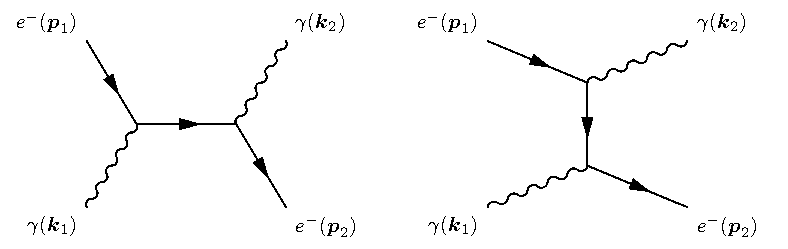
\includegraphics[width=.75\textwidth]{图/compton.pdf}
% \vspace{20pt}
%  \begin{fmffile}{compton_s}
%   \begin{fmfgraph*}(120,80)
%     \fmfleft{i1,i2}
%     \fmfright{o1,o2}
%     \fmflabel{$\gamma(\boldsymbol{k}_1)$}{i1}
%     \fmflabel{$e^-(\boldsymbol{p}_1)$}{i2}
%     \fmflabel{$e^-(\boldsymbol{p}_2)$}{o1}
%     \fmflabel{$\gamma(\boldsymbol{k}_2)$}{o2}
%     \fmf{boson}{i1,v1}
%     \fmf{fermion}{i2,v1}
%     \fmf{boson}{v2,o2}
%     \fmf{fermion}{v2,o1}
%     \fmf{fermion}{v1,v2}
%   \end{fmfgraph*}
% \end{fmffile} \qquad\qquad\qquad \begin{fmffile}{compton_t}
%   \begin{fmfgraph*}(120,80)
%     \fmfleft{i1,i2}
%     \fmfright{o1,o2}
%     \fmflabel{$\gamma(\boldsymbol{k}_1)$}{i1}
%     \fmflabel{$e^-(\boldsymbol{p}_1)$}{i2}
%     \fmflabel{$e^-(\boldsymbol{p}_2)$}{o1}
%     \fmflabel{$\gamma(\boldsymbol{k}_2)$}{o2}
%     \fmf{boson}{i1,v1}
%     \fmf{fermion}{v1,o1}
%     \fmf{fermion}{i2,v2}
%     \fmf{boson}{v2,o2}
%     \fmf{fermion}{v2,v1}
%   \end{fmfgraph*}
% \end{fmffile}
% \vspace{20pt}
\caption{}
\end{figure}
由费曼规则，我们可得：
\begin{equation}
\begin{split}
-i\mathcal{M}=&\bar{u}({p}_2)(-ie)\slashed{\varepsilon}^*({k}_2)\frac{i(\slashed{p}_1+\slashed{k}_1+m)}{(p_1+k_1)^2-m^2}\slashed{\varepsilon}({k}_1)(-ie)u({p}_1)\\&+\bar{u}({p}_2)(-ie)\slashed{\varepsilon}({k}_1)\frac{i(\slashed{p}_1-\slashed{k}_2+m)}{(p_1-k_2)^2-m^2}\slashed{\varepsilon}^*({k}_2)(-ie)u({p}_1)\\
&\hspace{-1.2cm}=-ie^2\bar{u}(p_2)\left[\frac{\slashed{\varepsilon}^*(k_2)(\slashed{p}_1+\slashed{k}_1+m)\slashed{\varepsilon}(k_1)}{(p_1+k_1)^2-m^2}+\frac{\slashed{\varepsilon}(k_1)(\slashed{p}_1-\slashed{k}_2+m)\slashed{\varepsilon}^*(k_2)}{(p_1-k_2)^2-m^2}\right]u(p_1)
\end{split}
\end{equation}
其中利用了$\gamma^\mu$矩阵的反对易关系以及各粒子的质量在壳条件。我们知道光子极化矢量必然正交与光子动量，则有$k_1\cdot\varepsilon_1=0,k_2\cdot\varepsilon_2=0$。此时我们还可以利用$u_1$的运动方程$(-\slashed{p}_1+m)u(p_1)=0$，则可得：
\begin{equation}
-i\mathcal{M}=-ie^2\bar{u}_2\Big(\frac{\slashed{\varepsilon}^*_2\slashed{k}_1\slashed{\varepsilon}_1+2\slashed{\varepsilon}^*_2p_1\cdot\varepsilon_1}{2p_1\cdot k_1}+\frac{\slashed{\varepsilon}_1\slashed{k}_2\slashed{\varepsilon}^*_2-2\slashed{\varepsilon}_1p_1\cdot\varepsilon^*_2}{2p_1\cdot k_2}\Big)u_1
\end{equation}

考虑非极化过程的自旋求和，对于电子而言我们已经在之前进行过讨论，而对于光子而言，我们则引用\eqref{eq:phopolsum}式可得光子极化矢量的求和条件$\sum_{r=1}^3\varepsilon^r_\mu{\varepsilon^*}^r_\nu=-\eta_{\mu\nu}$。且考虑初态粒子求平均，则有：
\begin{equation}
\begin{split}
\overline{|\mathcal{M}|}^2=\frac{e^4}{4}\eta_{\mu\rho}\eta_{\nu\sigma} \mathrm{tr}\Big[&\left(\frac{\gamma^\mu \slashed{k}_1\gamma^\nu+2\gamma^\mu p_1^\nu}{2p_1\cdot k_1}+\frac{\gamma^\nu \slashed{k}_2\gamma^\mu-2\gamma^\nu p_1^\mu}{2p_1\cdot k_2}\right)(\slashed{p}_1+m)\\
&\left(\frac{\gamma^\sigma \slashed{k}_1\gamma^\rho+2\gamma^\rho p_1^\sigma}{2p_1\cdot k_1}+\frac{\gamma^\rho \slashed{k}_2\gamma^\sigma-2\gamma^\sigma p_1^\rho}{2p_1\cdot k_2}\right)(\slashed{p}_2+m)\Big]
\end{split}
\end{equation}
我们利用四动量守恒可得如下关系：
\begin{align}
&p_2\cdot k_2=p_1\cdot k_1, &p_2\cdot k_1=p_1\cdot k_2 &\notag\\
&p_1\cdot p_2=m^2+p_1\cdot k_1-p_1\cdot k_2, &k_1\cdot k_2=p_1\cdot k_1&-p_1\cdot k_2
\end{align}
然后进行求迹并化简可得：
% \begin{small}
\begin{equation}
\overline{|\mathcal{M}|}^2=2e^4\left[\frac{p_1\cdot k_2}{p_1\cdot k_1}+\frac{p_1\cdot k_1}{p_1\cdot k_2}+2m^2\left(\frac{1}{p_1\cdot k_1}-\frac{1}{p_1\cdot k_2}\right)+m^4\left(\frac{1}{p_1\cdot k_1}-\frac{1}{p_1\cdot k_2}\right)^2\right]
\end{equation}
% \end{small}

对于Compton散射，我们通常考虑的实验室坐标系为初态电子的静止坐标系，即高能光子射击静止的靶电子。那么初态电子的四动量就可以表示为$p^\mu_1=(m,0,0,0)$，因此$p_1\cdot k=m\omega$，$\omega=k^0$为光子动量的类时分量，即光的角频率。而由靶心系中的四动量守恒我们可得Compton散射公式：
\begin{equation}
\omega_2=\frac{\omega_1}{1+\frac{\omega_1}{m}(1-\cos\theta)},\qquad \lambda'=\lambda+\lambda_\text{c}(1-\cos\theta)
\end{equation}
其中$\lambda_\text{c}=\frac{2\pi}{m}$为Compton波长，而$\lambda$为入射光波长，$\theta$则为入射光子与出射光子的夹角$\cos\theta=\frac{\boldsymbol{k}_1\cdot\boldsymbol{k}_2}{|\boldsymbol{k}_1||\boldsymbol{k}_2|}$。

而对于靶心系中的末态相空间，由\eqref{eq:dlips}式可得：
\begin{equation}
\begin{split}
\mathrm{d}Q_\text{LIPS}=&\frac{1}{4(2\pi)^2}\frac{\delta(|\boldsymbol{k}_2|-k_2^0){|\boldsymbol{k}_2|}^2\mathrm{d}|\boldsymbol{k}_2|\mathrm{d}\Omega}{\left|1-\frac{(\boldsymbol{k}_1-\boldsymbol{k}_2)\cdot\boldsymbol{k}_2}{p_2^0|\boldsymbol{k}_2|}\right|_{\boldsymbol{k}_2=k_2^0}\;k_2^0 p_2^0}=\frac{{k_2^0}^2\mathrm{d}\Omega}{4(2\pi)^2 \frac{p_2\cdot k_2}{k_2^0 p_2^0} k_2^0 p_2^0}\\
=&\frac{{k_2^0}^2\mathrm{d}\Omega}{16\pi^2mk_1^0}
\end{split}
\end{equation}
加上散射初态粒子的部分，我们可得微分截面为：
\begin{equation}
\frac{\mathrm{d}\sigma}{\mathrm{d}\Omega}=\frac{\overline{|\mathcal{M}|}^2{k_2^0}^2}{64\pi^2(p_1\cdot k_1)mk_1^0}
\end{equation}

利用Compton散射公式，并将振幅模方代入到微分截面中，我们可得：
\begin{equation}
\frac{\mathrm{d}\sigma}{\mathrm{d}\Omega}=\frac{\alpha^2}{2m^2}\left(\frac{\omega_2}{\omega_1}\right)^2\left(\frac{\omega_2}{\omega_1}+\frac{\omega_1}{\omega_2}-\sin^2\theta\right)
\end{equation}
上式即为光子的Compton散射微分截面，称为Klein-仁科公式。

我们知道电子经典半径为$r_e=\frac{\alpha}{m}$。则微分截面可写为仅关于入射光波长$\lambda$和散射角$\theta$的形式：
\begin{equation}
\frac{\mathrm{d}\sigma}{\mathrm{d}\Omega}=\frac{r_e^2}{2}\left[\frac{1+\cos^2\theta}{\left(1+\frac{\lambda_\text{c}}{\lambda}(1-\cos\theta)\right)^2}+\frac{\left(\frac{\lambda_\text{c}}{\lambda}(1-\cos\theta)\right)^2}{\left(1+\frac{\lambda_\text{c}}{\lambda}(1-\cos\theta)\right)^3}\right]
\end{equation}
那么对散射立体角积分即可得总的Compton散射截面：
\begin{equation}
\begin{split}
\sigma=&\pi r_e^2\left[\frac{4}{\left(\frac{\lambda_\text{c}}{\lambda}\right)^2}+\frac{2(1+\frac{\lambda_\text{c}}{\lambda})}{\left(1+2\frac{\lambda_\text{c}}{\lambda}\right)^2}-\frac{2+(2-\frac{\lambda_\text{c}}{\lambda})\frac{\lambda_\text{c}}{\lambda}}{\left(\frac{\lambda_\text{c}}{\lambda}\right)^3}\ln\left(1+2\frac{\lambda_\text{c}}{\lambda}\right)\right]
\end{split}
\end{equation}
如果当入射波波长相较于Compton波长极大时，$\frac{\lambda_\text{c}}{\lambda}\rightarrow0$，总截面则近似为：
\begin{equation}
\begin{split}
\sigma&\approx\pi r_e^2\left[\frac{8}{3}-\frac{16}{3}\frac{\lambda_\text{c}}{\lambda}+\frac{208}{15}\left(\frac{\lambda_\text{c}}{\lambda}\right)^2+\cdots\right]\\
&\approx\frac{8}{3}\pi r_e^2
\end{split}
\end{equation}
即在长波极限下，则Compton散射截面回归到经典的汤姆逊散射截面，符合量子力学的经典极限。

\subparagraph{正负电子对生成}
我们知道只要当两束光子的能量大于2个电子质量的时候，就可以相互作用从真空中产生一对正负电子对。该过程即为：
\[\gamma+\gamma\rightarrow e^+ + e^-\]
\begin{figure}[h]
\centering
	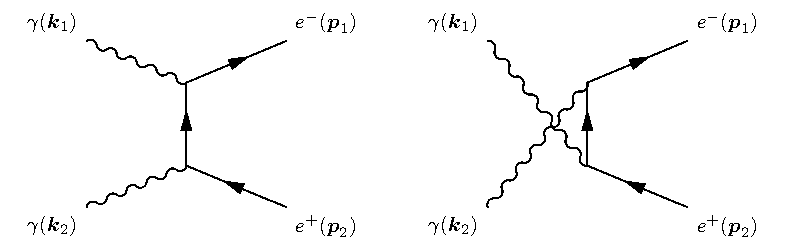
\includegraphics[width=.75\textwidth]{图/pair.pdf}
%  \vspace{20pt}
%  \begin{fmffile}{pair_t}
%   \begin{fmfgraph*}(120,80)
%     \fmfleft{i1,i2}
%     \fmfright{o1,o2}
%     \fmflabel{$\gamma(\boldsymbol{k}_2)$}{i1}
%     \fmflabel{$\gamma(\boldsymbol{k}_1)$}{i2}
%     \fmflabel{$e^+(\boldsymbol{p}_2)$}{o1}
%     \fmflabel{$e^-(\boldsymbol{p}_1)$}{o2}
%     \fmf{boson}{i1,v1}
%     \fmf{fermion}{o1,v1}
%     \fmf{boson}{i2,v2}
%     \fmf{fermion}{v2,o2}
%     \fmf{fermion}{v1,v2}
%   \end{fmfgraph*}
% \end{fmffile} \qquad\qquad\qquad\begin{fmffile}{pair_u}
%   \begin{fmfgraph*}(120,80)
%     \fmfleft{i1,i2}
%     \fmfright{o1,o2}
%     \fmflabel{$\gamma(\boldsymbol{k}_2)$}{i1}
%     \fmflabel{$\gamma(\boldsymbol{k}_1)$}{i2}
%     \fmflabel{$e^+(\boldsymbol{p}_2)$}{o1}
%     \fmflabel{$e^-(\boldsymbol{p}_1)$}{o2}
%     \fmf{boson,tension=0}{i1,v2}
%     \fmf{boson,tension=0}{i2,v1}
%     \fmf{phantom}{v1,i1}
%     \fmf{phantom}{v2,i2}
%     \fmf{fermion}{o1,v1}
%     \fmf{fermion}{v2,o2}
%     \fmf{fermion}{v1,v2}
%   \end{fmfgraph*}
% \end{fmffile}
% \vspace{20pt}
 \caption{}
\end{figure}
那么其散射振幅即为：
\begin{equation}
\begin{split}
-i\mathcal{M}=\bar{u}(p_1)(-ie)\slashed{\varepsilon}(k_1)\frac{i(\slashed{k}_1-\slashed{p}_1+m)}{(k_1-p_1)^2-m^2}\slashed{\varepsilon}(k_2)(-ie)v(p_2)\\
+\bar{u}(p_1)(-ie)\slashed{\varepsilon}(k_2)\frac{i(\slashed{k}_2-\slashed{p}_1+m)}{(k_2-p_1)^2-m^2}\slashed{\varepsilon}(k_1)(-ie)v(p_2)\\
=-ie^2\bar{u}_1\left(\frac{2\varepsilon_1\cdot p_1-\slashed{\varepsilon}_1\slashed{k}_1}{2k_1\cdot p_1}\slashed{\varepsilon}_2+\frac{2\varepsilon_2\cdot p_1-\slashed{\varepsilon}_2\slashed{k}_2}{2k_2\cdot p_1}\slashed{\varepsilon}_1\right)v_2
\end{split}
\end{equation}
与Compton散射的计算过程同理，我们可得非极化的振幅模方：
% \begin{small}
\begin{equation}
\overline{|\mathcal{M}|}^2=2e^2\left[\frac{p_1\cdot k_2}{p_1\cdot k_1}+\frac{p_1\cdot k_1}{p_1\cdot k_2}+2m^2\left(\frac{1}{p_1\cdot k_1}+\frac{1}{p_1\cdot k_2}\right)-m^4\left(\frac{1}{p_1\cdot k_1}+\frac{1}{p_1\cdot k_2}\right)^2\right]
\end{equation}
% \end{small}
可以看出，该振幅模方实际等同于将Compton散射振幅模方中的动量替换为$p_1\rightarrow-p_1$和$k_2\rightarrow-k_2$，且对$m^4$项加额外的负号。

对于该过程，我们则可选取质心系，那么我们可得动量的内积：
\begin{equation}
p_1\cdot k_1=m^2\frac{1-\beta\cos\theta}{1-\beta^2},\qquad p_1\cdot k_2=m^2\frac{1+\beta\cos\theta}{1-\beta^2}
\end{equation}
$\theta$角即为动量中心系的横向散射角，而$\beta=v$则为出射电子的相对论速度。由于选取的是质心系，因此两电子的速度相等，都可以用$\beta$来描述。由此我们可得末态相空间为：
\begin{equation}
\mathrm{d}Q_\text{LIPS}=\frac{\beta}{32\pi^2}\mathrm{d}\Omega
\end{equation}
因此微分截面可表为：
\begin{equation}
\frac{\mathrm{d}\sigma}{\mathrm{d}\Omega}=\frac{\overline{|\mathcal{M}|}^2(1-\beta^2)\beta}{256\pi^2m^2}
\end{equation}
代入振幅模方，可得正负电子对生成过程的微分截面：
\begin{equation}
\frac{\mathrm{d}\sigma}{\mathrm{d}\Omega}=\frac{\alpha^2(1-\beta^2)\beta}{4m^2}\left(\frac{1+\beta^2\cos^2\theta+2(1-\beta^2)}{1-\beta^2\cos^2\theta}-\frac{2(1-\beta^2)^2}{(1-\beta^2\cos^2\theta)^2}\right)
\end{equation}
对其积分，则可得正负电子对生成过程的总散射截面：
\begin{equation}
\sigma=\frac{\pi r_e^2}{2}(1-\beta^2)\left(2\beta(\beta^2-2)-(\beta^4-3)\ln\Big(\frac{1+\beta}{1-\beta}\Big)\right)
\end{equation}

\subparagraph{正负电子对湮灭} 而当一对正负电子对相遇时，则会相互湮灭，并将能量转化为光子。该过程即为：
\[e^+ + e^-\rightarrow \gamma+\gamma\]
\begin{figure}[h]
\centering
	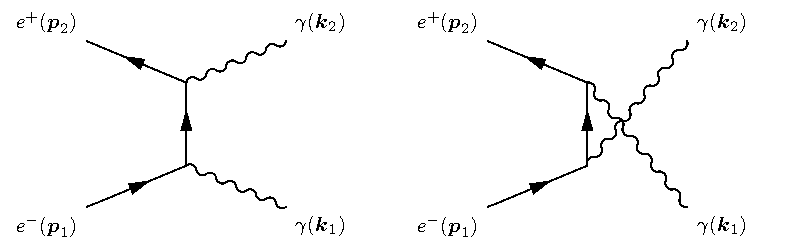
\includegraphics[width=.75\textwidth]{图/annihilation.pdf}
%  \vspace{20pt}
%  \begin{fmffile}{annihilation_t}
%   \begin{fmfgraph*}(120,80)
%     \fmfleft{i2,i1}
%     \fmfright{o2,o1}
%     \fmflabel{$\gamma(\boldsymbol{k}_1)$}{o1}
%     \fmflabel{$\gamma(\boldsymbol{k}_2)$}{o2}
%     \fmflabel{$e^-(\boldsymbol{p}_1)$}{i1}
%     \fmflabel{$e^+(\boldsymbol{p}_2)$}{i2}
%     \fmf{fermion}{i1,v1}
%     \fmf{boson}{o1,v1}
%     \fmf{fermion}{v2,i2}
%     \fmf{boson}{v2,o2}
%     \fmf{fermion}{v1,v2}
%   \end{fmfgraph*}
% \end{fmffile} \qquad\qquad\qquad\begin{fmffile}{annihilation_u}
%   \begin{fmfgraph*}(120,80)
%     \fmfleft{i2,i1}
%     \fmfright{o2,o1}
%     \fmflabel{$\gamma(\boldsymbol{k}_1)$}{o1}
%     \fmflabel{$\gamma(\boldsymbol{k}_2)$}{o2}
%     \fmflabel{$e^-(\boldsymbol{p}_1)$}{i1}
%     \fmflabel{$e^+(\boldsymbol{p}_2)$}{i2}
%     \fmf{boson,tension=0}{o1,v2}
%     \fmf{boson,tension=0}{o2,v1}
%     \fmf{phantom}{v1,o1}
%     \fmf{phantom}{v2,o2}
%     \fmf{fermion}{i1,v1}
%     \fmf{fermion}{v2,i2}
%     \fmf{fermion}{v1,v2}
%   \end{fmfgraph*}
% \end{fmffile}
% \vspace{20pt}
 \caption{}
\end{figure}
由于该过程实际上为正负电子对生成的逆过程，所以非极化振幅模方与此仅差一负号：
% \begin{small}
	\begin{equation}
	\overline{|\mathcal{M}|}^2=-2e^2\left[\frac{p_1\cdot k_2}{p_1\cdot k_1}+\frac{p_1\cdot k_1}{p_1\cdot k_2}+2m^2\left(\frac{1}{p_1\cdot k_1}+\frac{1}{p_1\cdot k_2}\right)-m^4\left(\frac{1}{p_1\cdot k_1}+\frac{1}{p_1\cdot k_2}\right)^2\right]
	\end{equation}
% \end{small}
同样我们选取质心系作为参考系。然而过程的初末态并不相同，则实际的散射截面关于入射粒子及末态相空间的部分则会不同：
\begin{equation}
\frac{\mathrm{d}\sigma}{\mathrm{d}\Omega}=\frac{\overline{|\mathcal{M}|}^2}{256\pi^2m^2\gamma\sqrt{\gamma^2-1}}
\end{equation}
其中$\gamma=\frac{\omega}{m}$为出射光频率与电子质量之比，也为初态电子的洛伦兹因子。且我们有：
\begin{equation}
p_1\cdot k_1=m^2(\gamma^2-\gamma\sqrt{\gamma^2-1}\cos\theta),\quad p_1\cdot k_2=m^2(\gamma^2+\gamma\sqrt{\gamma^2-1}\cos\theta)
\end{equation}
可得正负电子湮灭的微分截面为：
\begin{equation}
\frac{\mathrm{d}\sigma}{\mathrm{d}\Omega}=\frac{\alpha^2}{4m^2\gamma\sqrt{\gamma^2-1}}\left(\frac{2}{(\gamma^2-(\gamma^2-1)\cos^2\theta)^2}-\frac{\gamma^2+(\gamma^2-1)\cos^2\theta+2}{\gamma^2-(\gamma^2-1)\cos^2\theta}\right)
\end{equation}
那么总的散射截面为：
\begin{equation}
\sigma={\pi r_e^2}\left(\frac{1-2\gamma^2-2\gamma^4}{\gamma^4(\gamma^2-1)}\ln\left(\gamma+\sqrt{\gamma^2-1}\right)+\frac{1+\gamma^2}{\gamma^3\sqrt{\gamma^2-1}}\right)
\end{equation}
%\subsection*{极化散射过程与螺旋度结构}
%\subsubsection{极化费米子}
%\subsubsection{极化光子}


\section{QED辐射修正}
\subsection{QED单圈重整化}
当我们考虑QED的圈图修正时，则需要讨论重整化QED理论。那么我们可以定义裸的QED理论，同时有裸场、裸物理量与重整化场、重整化物理量的关系：
\begin{equation}
\psi_0=\sqrt{Z_\psi}\psi_r,\quad A_0^\mu=\sqrt{Z_A}A^\mu_r,\quad m_0=Z_m m_r,\quad e_0=Z_e e_r
\end{equation}
则重整化QED Lagrangian可以写为：
\begin{equation}
\mathscr{L}_\text{QED}=iZ_\psi\bar{\psi}_r\slashed{\partial}\psi_r- Z_m Z_\psi m_r \bar{\psi}_r\psi_r-\frac{1}{4}Z_A F_{\mu\nu}^r {F^r}^{\mu\nu}-e_r \sqrt{Z_A}Z_\psi Z_e \bar{\psi}_r \slashed{A}_r \psi_r
\end{equation}
此时我们可从此Lagrangian中得到重整化的3点函数和费米子传播子逆：
\begin{equation}
S^{-1}_r(p)=Z_\psi(\slashed{p}-m_0),\qquad\tilde{\Gamma}_r^\mu=\sqrt{Z_A}Z_\psi Z_e \gamma^\mu
\end{equation}
代入\eqref{eq:wardf}式的Ward恒等式中，并与树图层面的等式比较，易得：
\begin{equation}
Z_\psi\sqrt{Z_A}Z_e = Z_\psi,\qquad Z_e=Z_A^{-\frac{1}{2}}
\end{equation}
则重整化QED Lagrangian可改写为：
\begin{equation}
	\mathscr{L}_\text{QED}=iZ_\psi\bar{\psi}_r\slashed{\partial}\psi_r- Z_m Z_\psi m_r \bar{\psi}_r\psi_r-\frac{1}{4}Z_A F_{\mu\nu}^r {F^r}^{\mu\nu}-e_r Z_\psi \bar{\psi}_r \slashed{A}_r \psi_r
\end{equation}
%而光子场和费米子场的质量量纲分别为：
%\begin{equation}
%[A_\mu]=\frac{d}{2}-1,\qquad [\psi]=\frac{d-1}{2}
%\end{equation}
\subparagraph{电子自能}
要想求解重整化QED的$Z_\psi, Z_m$，则需要计算费米子的自能，而其中电子作为几乎只参与电磁相互作用的粒子，其自能基本上源自于纯的QED贡献，因此我们则考虑以电子为例费米子的QED重整化。考虑电子的2点格林函数，在单圈层面有如下费曼图，即为电子的自能项：
\begin{figure}[h]
\centering
% \begin{fmffile}{self_electron}
%     \begin{fmfgraph*}(120,100)
%        \fmfleft{i}
%        \fmfright{o}
%        \fmf{fermion,tension=1,label=$p$}{i,v1} 
%        \fmf{fermion,tension=1,label=$p$}{v2,o}
%        \fmf{boson,left,tension=0,label=${k}$}{v1,v2
%        }
%        \fmf{fermion,label=${k-p}$}{v1,v2
%        }
%     \end{fmfgraph*}
% \end{fmffile}
    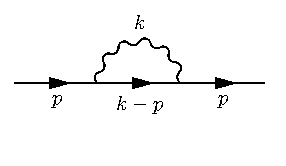
\includegraphics[scale=1.3]{图/self_electron.pdf}
\caption{}
\end{figure}
那么其单圈积分即为：
\begin{equation}
i\Sigma(p)=-e_0^2\int\frac{\mathrm{d}^dk}{(2\pi)^d}\frac{\gamma^\mu(\slashed{p}-\slashed{k}+m)\gamma^\nu}{(p-k)^2-m^2}\frac{(\eta_{\mu\nu}-(1-\xi)\frac{k_\mu k_\nu}{k^2})}{k^2}
\end{equation}
由费米子场量纲$[\psi]=\frac{d-1}{2}$及光子场量纲$[\phi]=\frac{d}{2}-1$可以推算得元电荷的量纲为$[e]=2-\frac{d}{2}$。当我们考虑$d$回归到4维时，我们可以将元电荷用能标参数化为$e_0=e\mu^{\frac{\epsilon}{2}}$。同时为了方便引用费曼积分公式，我们重新定义动量$k_\mu$的方向$k_\mu\rightarrow -k_\mu$，得：
% {\footnotesize 
\begin{equation}
	\begin{split}
i\Sigma(p)&=-e^2\mu^\epsilon\int\frac{\mathrm{d}^dk}{(2\pi)^d}\Big[\frac{\gamma^\mu(\slashed{p}+\slashed{k}+m)\gamma_\mu}{[(p+k)^2-m^2]k^2}-(1-\xi)\frac{\slashed{k}(\slashed{p}+\slashed{k}+m)\slashed{k}}{[(p+k)^2-m^2]k^4}\Big]\\
&=e^2\mu^\epsilon\int\frac{\mathrm{d}^dk}{(2\pi)^d}\Big[\frac{(d-\xi-1)\slashed{k}+(d+\xi-3)\slashed{p}+(1-d-\xi)m}{(k^2+2k\cdot p -m^2+p^2)k^2}+\frac{(1-\xi)2p\cdot k \slashed{k}}{(k^2+2k\cdot p -m^2+p^2)k^4}\Big]
	\end{split}
\end{equation}%}
由费曼积分公式\eqref{eq:loopint}式及其结果\eqref{eq:feyint}式可得：
\begin{equation}
i\Sigma(p)=e^2\mu^\epsilon \Big[I_{1,1}((d+\xi-3)\slashed{p}+(1-d-\xi)m)+(d-\xi-1)\gamma_\mu I^\mu_{1,1}+2(1-\xi)p_\mu\gamma_\nu I^{\mu\nu}_{1,2}\Big]
\end{equation}
进一步化简，可得电子自能：
%\begin{multline}
%\Sigma(p)=\frac{e^2}{16\pi^2}\Big[((1+\xi-\epsilon)\slashed{p}+(\epsilon-3-\xi)m)\Gamma(\frac{\epsilon}{2})\int_0^1\mathrm{d}x\left(\frac{4\pi\mu^2}{\Omega(x)}\right)^{\frac{\epsilon}{2}}\\-(3-\epsilon-\xi)\slashed{p}\Gamma(\frac{\epsilon}{2})\int_0^1\mathrm{d}x\,x\left(\frac{4\pi\mu^2}{\Omega(x)}\right)^{\frac{\epsilon}{2}}\\-(1-\xi)(2p^2 \slashed{p}\int_0^1\mathrm{d}x\frac{x^3}{\Omega}+{\slashed{p}}\Gamma(\frac{\epsilon}{2})\int_0^1\mathrm{d}x\,x\Big(\frac{4\pi\mu^2}{\Omega}\Big)^{\frac{\epsilon}{2}})\Big]
%\end{multline}
\begin{multline}
\Sigma(p)=\frac{e^2}{8\pi^2}\Big[\frac{(2\xi-1)\slashed{p}-(\xi+3)m}{\epsilon}-\frac{\slashed{p}}{2}+m+\Big((\xi-\frac{1}{2})\slashed{p}-\frac{\xi+3}{2}m\Big)\ln \frac{4\pi}{e^\gamma}\\+\int_0^1\mathrm{d}x\Big([(\xi-2)x+\frac{\xi+1}{2}]\slashed{p}-\frac{\xi+3}{2}m\Big)\ln\frac{\mu^2}{\Omega}-(1-\xi)p^2 \slashed{p}\int_0^1\mathrm{d}x\frac{x^3}{\Omega}\Big]
\end{multline}
其中：\begin{equation}
	\Omega=x[(x-1)p^2+m^2]
\end{equation}
\begin{itemize}
\item 当我们选取费曼规范时，即$\xi=1$，则电子自能为：
\end{itemize}
\begin{equation}
\Sigma(p)=\frac{e^2}{8\pi^2}\Big[\frac{\slashed{p}-4m}{\epsilon}+(\frac{\slashed{p}}{2}-2m)\ln 4\pi e^{-\gamma}+m-\frac{\slashed{p}}{2}+\int_0^1\mathrm{d}x[\slashed{p}(1-x)-2m]\ln\frac{\mu^2}{x[(x-1)p^2+m^2]}\Big]
\end{equation}

\begin{itemize}
	\item 当我们选取朗道规范时，即$\xi=0$，则电子自能为：
\end{itemize}
\begin{multline}
	\Sigma(p)=\frac{e^2}{8\pi^2}\Big[\frac{-\slashed{p}-3m}{\epsilon}-\frac{1}{2}\Big(\slashed{p}+3m\Big)\ln 4\pi e^{-\gamma}+m-\slashed{p}\Big(\frac{(p^2-m^2)^2}{p^4}\ln\frac{m^2}{p^2-m^2}\\-2\frac{m^2}{p^2}+\frac{7}{2}\Big)-\int_0^1\mathrm{d}x\Big([2x-\frac{1}{2}]\slashed{p}+\frac{3}{2}m\Big)\ln\frac{\mu^2}{x[(x-1)p^2+m^2]}\Big]
\end{multline}
当我们已经计算出电子自能时，我们则可以考虑对电子场的重整化。即考虑电子的裸2点格林函数\(G_0(x_1,x_2)\sim\langle0|{\psi_0}\bar{\psi}_0|0\rangle\)，代入重整化的电子场后，可得裸2点格林函数与重整化2点格林函数的关系\({G}_r=\frac{1}{Z_\psi}G_0\)，那么可得：
\begin{equation}
{\tilde{G}}_r=\frac{1}{Z_\psi}\Big[\frac{i}{\slashed{p}-Z_m m_r}+\frac{i}{\slashed{p}-m}i\Sigma(p)\frac{i}{\slashed{p}-m}+\mathcal{O}(e^4)+\cdots\Big]
\end{equation}
代入重整化系数\(Z_\psi=1+\delta_\psi, Z_m=1+\delta_m\)，可得：
\begin{equation}
\begin{split}
{\tilde{G}}_r&=\frac{1}{1+\delta_\psi}\Big[\frac{i}{\slashed{p}-m_r-\delta_m m_r}+\frac{i}{\slashed{p}-m_r}i\Sigma(p)\frac{i}{\slashed{p}-m_r}+\mathcal{O}(e^4)+\cdots\Big]\\
&=\frac{i}{\slashed{p}-m_r}+\frac{i}{\slashed{p}-m_r}i\Big(\Sigma(p)+\delta_\psi(\slashed{p}-m_r)-\delta_m m_r\Big)\frac{i}{\slashed{p}-m_r}+\mathcal{O}(e^4)+\cdots
\end{split}
\end{equation}
我们考虑选取费曼规范，并选择最小差值(MS)重整化方案，将自能中的发散项抵消掉，便可求解得：
\begin{equation}
\delta^\text{MS}_\psi=-\frac{e^2}{8\pi^2\epsilon}=-\frac{\alpha}{2\pi\epsilon},\qquad\delta_m^\text{MS}=-\frac{3e^2}{8\pi^2\epsilon}=-\frac{3\alpha}{2\pi\epsilon}
\label{eq:qedferren}
\end{equation}
则我们最终得到在费曼规范下的首一阶电子场重整化和电子质量重整化结果：
\begin{equation}
\psi_0=\psi_r\left(1-\frac{\alpha}{2\pi\epsilon}\right)^\frac{1}{2},\qquad m_0=m_r\left(1-\frac{3\alpha}{2\pi\epsilon}\right)
\end{equation}

带入回电子传播子中，我们可得：
\begin{equation}
    S(p)=\frac{i}{\slashed{p}-m+\Sigma_r(p)}
\end{equation}
其中的质量修正项$\Sigma_r(p)=\Sigma(p)+\delta_\psi(\slashed{p}-m_r)-\delta_m m_r$为消去了发散项的电子自能。在最小差值(MS)方案下为：
\begin{equation}
    \Sigma^\text{MS}_r(p)=\frac{\alpha}{2\pi}\Big[m-\frac{\slashed{p}}{2}+\int_0^1\mathrm{d}x[\slashed{p}(1-x)-2m]\ln\frac{4\pi\mu^2e^{-\gamma}}{x[(x-1)p^2+m^2]}\Big]
\end{equation}
而当我们考虑在壳重整化时，我们有：
\begin{equation}
    \Sigma^\text{OS}_r(m_\text{pole})=0,\qquad \frac{\mathrm{d}\Sigma^\text{OS}_r(\slashed{p})}{\mathrm{d}\slashed{p}}\Big|_{\slashed{p}=m_\text{pole}}=0
\end{equation}
%\Big[\Sigma(\slashed{p})+\delta^\text{OS}_\psi(\slashed{p}-m_\text{pole})-m_\text{pole}\delta^\text{OS}_m\Big]\Big|_{\slashed{p}=m_\text{pole}}=0
可得：
\begin{equation}
    \delta^\text{OS}_m=\frac{\Sigma(m_\text{pole})}{m_\text{pole}},\qquad \delta^\text{OS}_\psi=-\frac{\mathrm{d}\Sigma^\text{OS}(\slashed{p})}{\mathrm{d}\slashed{p}}\Big|_{\slashed{p}=m_\text{pole}}
\end{equation}
代入费曼规范下的电子自能，我们可得：
\begin{align}
    \delta^\text{OS}_m&=-\frac{\alpha}{2\pi}\Bigg[\frac{3}{\epsilon}+2+\frac{3}{2}(\ln{4\pi}-\gamma)+\frac{3}{2}\ln\left(\frac{\mu^2}{m_\text{pole}^2}\right)\Bigg]\notag\\
    \delta^\text{OS}_\psi&=-\frac{\alpha}{2\pi}\Bigg[\frac{1}{\epsilon}+2+\frac{1}{2}(\ln{4\pi}-\gamma)+\frac{1}{2}\ln\left(\frac{\mu^2}{m_\text{pole}^2}\right)+2\ln\delta\Bigg]
\end{align}
其中$\delta\rightarrow 0$为引入的无穷小量。那么此时在壳方案下，我们可得电子质量修正项：
\begin{equation}
     \Sigma^\text{OS}_r(p)=\frac{\alpha}{2\pi}\Bigg[5(m-\frac{\slashed{p}}{2})+\int_0^1\mathrm{d}x[\slashed{p}(1-x)-2m]\ln\frac{m^2_\text{pole}}{x[(x-1)p^2+m^2]} -2(\slashed{p}-m)\ln\delta \Bigg]
\end{equation}
我们看到质量修正项完全独立于能标$\mu$，虽然该修正项中有发散项，但是当$\slashed{p}=m$时，修正项恒为0，则确保了电子的质量固定在极点质量上。
若我们考虑对$\overline{\text{MS}}$方案的修正项在极点质量处的取值$m(\mu)=m_\text{pole}+\Sigma_r^{\overline{\text{MS}}}(m_\text{pole})$，则可得电子极点质量与跑动质量之间的关系：
\begin{equation}
    m(\mu)=m_\text{pole}\left[  1-\frac{\alpha}{4\pi}\left(4+3\ln\frac{\mu^2}{m_\text{pole}^2}\right) +\mathcal{O}(\alpha^2)+\cdots\right]
\end{equation}

\subparagraph{真空极化}
考虑光子场的重整化$Z_A$时，我们则需要计算光子的自能，则单圈层面的光子2点格林函数可表示为费曼图~\ref{self_photon}。
\begin{figure}[h]
\centering
% \begin{fmffile}{self_photon}
%     \begin{fmfgraph*}(120,80)
%        \fmfleft{i}
%        \fmfright{o}
%        \fmf{boson,tension=1,label=$k$}{i,v1} 
%        \fmf{boson,tension=1,label=$k$}{v2,o}
%        \fmf{fermion,left,tension=0.4,label=${p}$}{v1,v2
%        }
%        \fmf{fermion,left,tension=0.4,label=${p-k}$}{v2,v1
%        }
%     \end{fmfgraph*}
% \end{fmffile}
	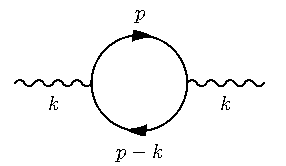
\includegraphics[scale=1.2]{图/self_photon.pdf}
 \caption{}
 \label{self_photon}
\end{figure}
此过程可看出光子将真空极化并使其生成一对正负费米子对，然后正负费米子对再湮灭产生能量相等的光子。此过程我们可以用自能表示为：
\begin{equation}
\Pi^{\mu\nu}(k)=-\int\frac{\mathrm{d}^d p}{(2\pi)^d}\sum_{\text{helicity}}(-ie_0\gamma^\mu)\frac{ i}{\slashed{p}-m}(-ie_0\gamma^\nu)\frac{ i}{\slashed{p}-\slashed{k}-m}
\end{equation}
对于内线费米子的螺旋度求和，即可以转换为旋量空间的求迹，则有：
\begin{equation}
	\Pi^{\mu\nu}(k)=-e_0^2\int\frac{\mathrm{d}^d p}{(2\pi)^d}\frac{\mathrm{tr}[\gamma^\mu(\slashed{p}+m)\gamma^\nu (\slashed{p}-\slashed{k}+m)]}{(p^2-m^2)((p-k)^2-m^2)}
\end{equation}
我们通过求迹公式，可得：
\begin{equation}
	\Pi^{\mu\nu}(k)=-4e_0^2\int\frac{\mathrm{d}^d p}{(2\pi)^d}\frac{2p^\mu p^\nu +p^\mu k^\nu+p^\nu k^\mu+(m^2-p^2-p\cdot k)\eta^{\mu\nu}}{(p^2-m^2)(p^2+2p\cdot k+k^2-m^2)}
\end{equation}
将内线动量反向\(p\rightarrow -p\)，则可利用费曼积分公式，求得：
% {\small
\begin{equation}
	\Pi^{\mu\nu}(k^2)=-4e_0^2\Big(2I^{\mu\nu}_{1,1}+k^\mu I^\nu_{1,1}+k^\nu I^\mu_{1,1}+\eta^{\mu\nu}(m^2I_{1,1}-{I^\alpha_\alpha}_{1,1}-k_\alpha I^\alpha_{1,1})\Big)
\end{equation}%}
其中
\begin{equation}
    \Omega=m^2+(x^2-x)k^2
\end{equation}
对于内部指标缩并的项${I^\alpha_\alpha}_{1,1}$，度规缩并为$\eta_{\mu\nu}\eta^{\mu\nu}=d=4-\epsilon$，再利用性质$x\Gamma(x)=\Gamma(x+1)$，可得其中一部分为：
\begin{equation}
    2I^{\mu\nu}_{1,1}-\eta^{\mu\nu}{I^\alpha_\alpha}_{1,1}=\frac{i}{(4\pi)^2}\int_0^1\mathrm{d}x\left(\frac{\Omega}{4\pi}\right)^{-\frac{\epsilon}{2}}\Gamma(\frac{\epsilon}{2})[x^2(2k^\mu k^\nu-\eta^{\mu\nu}k^2)-\eta^{\mu\nu}\Omega]
\end{equation}
然后可得另一部分：
\begin{equation}
    k^\mu I^\nu_{1,1}+k^\nu I^\mu_{1,1}-\eta^{\mu\nu}k_\alpha I^\alpha_{1,1} = -\frac{i}{(4\pi)^2}\Gamma(\frac{\epsilon}{2})\int_0^1\mathrm{d}x \;x \left(\frac{\Omega}{4\pi}\right)^{-\frac{\epsilon}{2}}(2k^\mu k^\nu-\eta^{\mu\nu}k^2)
\end{equation}
综合可得：
% {\small
\begin{equation}
    \Pi^{\mu\nu}(k)=-4e_0^2\frac{i}{(4\pi)^2}\Gamma(\frac{\epsilon}{2})\int_0^1\mathrm{d}x\left(\frac{\Omega}{4\pi}\right)^{-\frac{\epsilon}{2}}\Big[(x^2-x)(2k^\mu k^\nu-\eta^{\mu\nu}k^2)+\eta^{\mu\nu}(m^2-\Omega)\Big]
\end{equation}%}
代入$\Omega$以及$e_0=e\mu^\frac{\epsilon}{2}$，得光子自能：
\begin{equation}
    \Pi^{\mu\nu}(k)=\frac{ie^2}{2\pi^2}\left(\eta^{\mu\nu}-\frac{k^\mu k^\nu}{k^2}\right)\Gamma(\frac{\epsilon}{2})\int_0^1\mathrm{d}x\left(\frac{\Omega}{4\pi\mu^2}\right)^{-\frac{\epsilon}{2}}(\Omega-m^2)
\end{equation}
我们很容易看出，光子自能包含了横向投影的部分，因此有：
\begin{equation}
k_\mu \Pi^{\mu\nu}(k^2)=0
\end{equation}
这意味着即使考虑高阶修正光子也依然保持横向极化，使得光子并没有带上额外的质量。

再令$\epsilon$趋于0，可得：
% {\small
\begin{equation}
    \Pi^{\mu\nu}(k)={ie^2}k^2\left(\eta^{\mu\nu}-\frac{k^\mu k^\nu}{k^2}\right)\left(-\frac{1}{6\pi^2\epsilon}+\frac{1}{12\pi^2}\ln\frac{e^\gamma}{4\pi}-\frac{1}{2\pi^2}\int_0^1\mathrm{d}x(x-1)x\ln\frac{\Omega(x)}{\mu^2}\right)
\end{equation}%}

我们有裸光子场的2点格林函数\(D_{\mu\nu}\sim\langle0|{{A_0}_\mu}{A_0}_\nu|0\rangle\)，因此我们可得重整化2点光子场格林函数：
\begin{equation}
    D^r_{\mu\nu}(k)=\frac{1}{Z_A}\left[D_{\mu\nu}+D_{\mu\alpha}\Pi^{\alpha\beta}(k^2, e^2)D_{\beta\nu}+\mathcal{O}(e^4)+\cdots\right]
\end{equation}
由于光子自能可写成：
\begin{equation}
    \Pi^{\alpha\beta}(k^2, e^2)={ie^2}k^2\left(\eta^{\alpha\beta}-\frac{k^\alpha k^\beta}{k^2}\right)\Pi(k^2,\mu)
\end{equation}
那么我们可以使用朗道规范，光子传播子则为$D_{\mu\nu}=\frac{-i}{k^2}(\eta_{\mu\nu}-\frac{k_\mu k_\nu}{k^2})$。利用横向投影算符的性质，我们也可以将光子场格林函数也可写成几何级数形式：
\begin{align}
    D^r_{\mu\nu}(k)=&\frac{1}{Z_A}\frac{-i}{k^2}\left(\eta_{\mu\nu}-\frac{k_\mu k_\nu}{k^2}\right)\sum_{n=0}\left(e^2\Pi(k^2,\mu)\right)^n\notag\\
    &=\frac{1}{Z_A[1-e^2\Pi(k^2,\mu)]}\frac{-i}{k^2}\left(\eta_{\mu\nu}-\frac{k_\mu k_\nu}{k^2}\right)
\end{align}
令光子场重整化系数为$Z_A=1+\delta_A$，若使用最小差值方案重整化，那么我们可得：
\begin{equation}
    \delta_A=-\frac{e^2}{6\pi^2\epsilon}
\end{equation}
即：
\begin{equation}
    A_0^\mu=A^\mu\left(1-\frac{2\alpha}{3\pi\epsilon}\right)^\frac{1}{2}
\end{equation}
%带入回到光子传播子中
%\begin{equation}
%    D^r_{\mu\nu}(k)=\frac{-i}{k^2}\left(\eta_{\mu\nu}-\frac{k_\mu k_\nu}{k^2}\right)\left(1+\frac{e^2}{12\pi^2}\ln\frac{e^\gamma}{4\pi}-\frac{e^2}{2\pi^2}\int_0^1\mathrm{d}x(x-1)x\ln\frac{m^2+x(x-1)k^2}{\mu^2} \right)
%\end{equation}


%对于光子传播子，我们可以对其作傅里叶变换

\subparagraph{QED中的$\beta$函数}
由于我们已经得到了光子场重整化系数$Z_A$，我们可以通过Ward恒等式得到电荷重整化系数$Z_e=1/\sqrt{Z_A}$，最终我们解出QED中所有的重整化系数：
\begin{equation}
    Z_\psi=1-\frac{e^2}{8\pi^2\epsilon},\qquad Z_A=1-\frac{e^2}{6\pi^2\epsilon}, \qquad Z_m =1-\frac{3e^2}{8\pi^2\epsilon}, \qquad Z_e=1+\frac{e^2}{12\pi^2\epsilon}
\end{equation}

那么裸电荷表为：
\begin{equation}
    e_0= e\mu^{\frac{\epsilon}{2}}Z_e=e\mu^{\frac{\epsilon}{2}}\left(1+\frac{e^2}{12\pi^2\epsilon}\right)
\end{equation}
考虑：
\begin{equation}
    0=\mu\frac{\mathrm{d}}{\mathrm{d}\mu}e_0=\mu\frac{\mathrm{d}e}{\mathrm{d}\mu}\mu^{\frac{\epsilon}{2}}\left(1+\frac{e^2}{12\pi^2\epsilon}\right)+e\frac{\epsilon}{2}\mu^{\frac{\epsilon}{2}}\left(1+\frac{e^2}{12\pi^2\epsilon}\right)+\mu^{\frac{\epsilon}{2}}\frac{e^2}{6\pi^2\epsilon}\mu\frac{\mathrm{d}e}{\mathrm{d}\mu}
\end{equation}
那么最终另$\epsilon\rightarrow0$，我们可求解得QED的$\beta(e)$函数：
\begin{equation}
    \beta(e)=\mu\frac{\mathrm{d}e}{\mathrm{d}\mu}=\frac{e^3}{12\pi^2}
\end{equation}
则QED的跑动耦合常数即为：
\begin{equation}
    e^2(\mu)=\frac{e_\Lambda^2}{1-\frac{e_\Lambda^2}{6\pi^2}\ln\frac{\mu}{\Lambda}}
\end{equation}
或写为跑动精细结构常数：
\begin{equation}
    \alpha(\mu)=\frac{\alpha_\Lambda}{1-\frac{2\alpha_\Lambda}{3\pi}\ln\frac{\mu}{\Lambda}}
\end{equation}
由于QED的$\beta$-函数大于0，因此在低能标处QED不会出现渐近自由的现象，而在高能标时QED则会出现朗道极点。由我们现有的实验可知，在能标处于电子质量这个尺度的时候，精细结构常数大约是$\frac{1}{137}$。那么以此推算，我们可得QED朗道极点的能标大约为$\Lambda_\text{QED}\sim m_e e^{204\pi}\approx10^{283}$ eV。可以看出在目前实验观测范围内，所处的能标离$\Lambda_\text{QED}$还非常的遥远，因此在QED中使用微扰展开基本不会出现问题，同时该结果也符合我们对电磁相互作用的直觉。

%\subsection{QED红外发散}
\subparagraph{电子反常磁矩}
在之前的讨论中，我们已经对电磁相互作用的耦合常数进行了重整化。然而这并不代表电磁相互作用中的高阶效应已经考虑完备，实际上我们还需要考虑来自电子内部自旋的量子修正。那么我们知道电子参与相互作用时，其自旋的性质表现在磁矩上，因此电子的磁矩将会受到量子修正的影响。而有经典电动力学可知，磁矩由电流决定。则我们考虑如下电子流，中途外部电磁场于其发生相互作用的情形，而其单圈级别的作用过程可描述为费曼图~\ref{anomalous_mag}。
\begin{figure}[h]
\centering
% \begin{fmffile}{anomalous_mag}
%       \begin{fmfgraph*}(80,100)
%     \fmfleft{x2,x1}
%     \fmfright{x3}
%     \fmf{boson,t=1,label=$~~~~~~k$}{x3,v}
%     \fmf{fermion,label=$p_1$}{x2,v1}
%     \fmf{plain,t=1.3,label=$\!\!p_1-q$}{v1,v}
%         \fmf{plain,t=1.3,label=$\!\!p_2-q$}{v,v2}
%     \fmf{fermion,label=$p_2$}{v2,x1}
%         \fmffreeze
%     \fmf{boson,left=0.36,label=$q$,l.s=left}{v1,v2}
%   \end{fmfgraph*}
% \end{fmffile}
    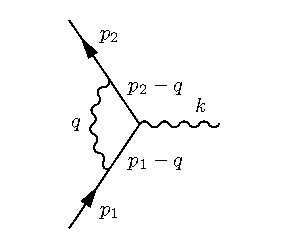
\includegraphics[scale=1.3]{图/anomalous_mag.pdf}
    \caption{}
    \label{anomalous_mag}
\end{figure}
那么该单圈电子流在费曼规范下可表示为：
% {\small
\begin{equation}
    J_{(1)}^\mu=\bar{u}(p_2)\Bigg[\int\frac{\mathrm{d}^4q}{(2\pi)^4}(-ie_0\gamma^\beta)\frac{i}{\slashed{p}_2-\slashed{q}-m}(-ie_0\gamma^\mu)\frac{i}{\slashed{p}_1-\slashed{q}-m}(-i_0e\gamma^\alpha)\frac{-i\eta_{\alpha\beta}}{q^2}\Bigg]u(p_1)
\end{equation}%}
此时考虑单圈级别的电流可以表示为$J_{(1)}^\mu=-ie_0\bar{u}(p_2)\Gamma_{(1)}^\mu u(p_1)$的普适形式，那么只考虑中间的顶点函数部分：
% {\small
\begin{align}
    \Gamma_{(1)}^\mu=&-ie_0^2\int\frac{\mathrm{d}^dq}{(2\pi)^d}\frac{\gamma_a(\slashed{p}_2-\slashed{q}+m)\gamma^\mu(\slashed{p}_1-\slashed{q}+m)\gamma^\alpha}{q^2[(p_2-q)^2-m^2][(p_1-q)^2-m^2]}\notag\\
    =&-ie_0^2\int\frac{\mathrm{d}^dq}{(2\pi)^d}\frac{[2(p_2-q)_\alpha-(\slashed{p}_2-m-\slashed{q})\gamma_\alpha]\gamma^\mu[2(p_1-q)^\alpha-\gamma^\alpha(\slashed{p}_1-m-\slashed{q})]}{q^2[(p_2-q)^2-m^2][(p_1-q)^2-m^2]}
\end{align}%}
由于考虑外线电子为是实的在壳电子，则有$\slashed{p}_2-m=0$，$\slashed{p}_1-m=0$，且考虑动量$q$反向，可得：
\begin{equation}
    \Gamma_{(1)}^\mu=-ie_0^2\int\frac{\mathrm{d}^dq}{(2\pi)^d}\frac{(2(p_2+q)_\alpha-\slashed{q}\gamma_\alpha)\gamma^\mu(2(p_1+q)^\alpha-\gamma^\alpha \slashed{q})}{q^2[q^2+2q\cdot p_2+p_2^2-m^2][q^2+2q\cdot p_1+p_1^2-m^2]}\notag\\
    %=e^2\int\frac{\mathrm{d}^dq}{(2\pi)^d}\frac{}{q^2[(p_2+q)^2-m^2][(p_1+q)^2-m^2]}
\end{equation}
对于分子部分，我们利用$\gamma_\alpha\gamma^\mu\gamma^\alpha=(2-d)\gamma^\mu$，且利用反对易关系，有：
% {\small
\begin{align}
&(2(p_2+q)_\alpha-\slashed{q}\gamma_\alpha)\gamma^\mu(2(p_1+q)^\alpha-\gamma^\alpha \slashed{q})\notag\\
    =&4\gamma^\mu(p_2+q)\cdot(p_1+q)-2\slashed{q}\gamma_\alpha\gamma^\mu(p_1+q)^\alpha-2(p_2+q)_\alpha\gamma^\mu\gamma^\alpha \slashed{q}+\slashed{q}\gamma_\alpha\gamma^\mu\gamma^\alpha \slashed{q}\notag\\
    =&4\gamma^\mu(p_2+q)\cdot(p_1+q)-4q^2\gamma^\mu-2\slashed{q} \slashed{p}_1\gamma^\mu-2\gamma^\mu \slashed{p}_2\slashed{q}+2(2-d)\slashed{q} q^\mu-(2-d)q^2 \gamma^\mu\notag\\
    =&\gamma^\mu [4(p_2\cdot p_1 + p_2\cdot q +q\cdot p_1)-(2-d)q^2]+2(2-d)\slashed{q} q^\mu-2\slashed{q} \slashed{p}_1\gamma^\mu-2\gamma^\mu \slashed{p}_2\slashed{q}\notag\\
    =&\gamma^\mu [4p_2\cdot p_1 + 4q\cdot(p_2 + p_1)-(2-d)q^2]+2(2-d)\slashed{q} q^\mu+4m q^\mu-4\slashed{q}(p_1+p_2)^\mu\notag\\
    =&4\gamma^\mu p_1\cdot p_2 + 4q^\nu[\gamma^\mu(p_1+p_2)_\nu-\gamma_\nu(p_1+p_2)^\mu+{m}\delta_\nu^\mu]+(2-d)q^\nu q^\rho[2\gamma_\rho\delta_\nu^\mu-\gamma^\mu\eta_{\nu\rho}] 
\end{align}%}
那么代入回积分中，我们可以引用费曼积分将其写为：
\begin{multline}
        \Gamma_{(1)}^\mu=-ie_0^2\Big[4\gamma^\mu p_1\cdot p_2 I_{1,1,1}+ 4I_{1,1,1}^\nu[\gamma^\mu(p_1+p_2)_\nu-\gamma_\nu(p_1+p_2)^\mu+{m}\delta_\nu^\mu]\\+(2-d)I_{1,1,1}^{\nu\rho}[2\gamma_\rho\delta_\nu^\mu-\gamma^\mu\eta_{\nu\rho}]    \Big]
\end{multline}
由于其中的单圈积分$I_{1,1,1}\sim \int\frac{\mathrm{d}q}{q^3}$，那么可以预见当内线动量$q\rightarrow0$时，圈积分则会出现发散。此时情况不同于内线动量$p\rightarrow\infty$时出现的发散，因此我们称之为\emph{红外发散}。

我们可以通过费曼积分公式，计算得：
% {\footnotesize
\begin{align}
I_{1,1,1}=&-\frac{i}{32\pi^2}\int_0^1\frac{\mathrm{d}x}{\Delta(x)}\ln\frac{\Delta(x)}{\epsilon^2}+\mathcal{O}(\epsilon),\qquad I_{1,1,1}^\mu=(p_1+p_2)^\mu\frac{i}{32\pi^2}\int_0^1\frac{\mathrm{d}x}{\Delta(x)}\\
I_{1,1,1}^{\mu\nu}=&\frac{i\eta^{\mu\nu}}{32\pi^2}\int_0^1 u\,\mathrm{d}u\int_0^1 x\,\mathrm{d}x\;\Gamma(\frac{\epsilon}{2})\left(\frac{u^2\Delta(x)}{4\pi}\right)^{-\frac{\epsilon}{2}}\notag\\&-\frac{i}{128\pi^2}\Big[(p_1+p_2)^\mu(p_1+p_2)^\nu\int_0^1\frac{\mathrm{d}x}{\Delta(x)}+(p_1-p_2)^\mu(p_1-p_2)^\nu\int_0^1\frac{x^2\mathrm{d}x}{\Delta(x)}\Big]
%\begin{split}
%
%\end{split}
\end{align}%}
%\frac{\eta^{\mu\nu}}{(d-2)^2\mu^\epsilon}\Big[\frac{i}{8\pi^2\epsilon}-\frac{i}{16\pi^2}\Big(\int_0^1\mathrm{d}x\ln\frac{\Omega(x)}{\mu^2}+\ln\frac{e^\gamma}{4\pi}\Big)+\mathcal{O}(\epsilon)\Big]
其中:
\begin{equation}
\Delta(x)=m^2-\frac{1}{4}(1-x^2)k^2,\qquad k^\mu=p^\mu_2-p^\mu_1
\end{equation}

此时对于两个外线电子而言，我们有狄拉克方程$(\slashed{p}_1-m)u(p_1)=0$，$\bar{u}(p_2)(\slashed{p}_2-m)=0$，可得：
\begin{align}
m\gamma^\mu u(p_1)=\gamma^\mu\gamma^\nu {p_1}_\nu u(p_1) =(p_1^\mu-i\sigma^{\mu\nu}{p_1}_\nu)u(p_1)\\
m \bar{u}(p_2)\gamma^\mu=\bar{u}(p_2){p_2}_\nu\gamma^\nu\gamma^\mu   =\bar{u}(p_2)(p_2^\mu+i\sigma^{\mu\nu}{p_2}_\nu)
\end{align}
然后在上式1式的左侧乘上$\bar{u}(p_2)$，在上式2式的右侧乘上$u(p_1)$，再将两式相加可得：
\begin{equation}
\bar{u}(p_2)\gamma^\mu u(p_1)=\bar{u}(p_2)\Big(\frac{(p_1+p_2)^\mu}{2m}-\frac{i\sigma^{\mu\nu}}{2m}(p_1-p_2)_\nu\Big) u(p_1)
\end{equation}
此式称为Gordon恒等式。通过此式我们可得：
\begin{equation}
(p_1+p_2)^\mu=2m\gamma^\mu +i\sigma^{\mu\nu}(p_1-p_2)_\nu
\end{equation}

综合以上结果，再带入回电流中的顶点函数项，我们可得：
\begin{multline}
\Gamma_{(1)}^\mu=e^2\Big[ \frac{i\sigma^{\mu\nu}}{16\pi^2}k_\nu\int_0^1\frac{\mathrm{d}x}{\Delta(x)}+\gamma^\mu\Big(\frac{1}{8\pi^2\epsilon}-\frac{p_1\cdot p_2}{8\pi^2}\int_0^1\frac{\mathrm{d}x}{\Delta(x)}\ln\frac{\Delta(x)}{\epsilon^2}\\
-\frac{1}{16\pi^2}\int_0^1\mathrm{d}x\ln\frac{\Delta(x)e^\gamma}{4\pi\mu^2}+\frac{p_1\cdot p_2}{32\pi^2}\int_0^1\frac{7+x^2}{\Delta(x)}\mathrm{d}x+\frac{m^2}{32\pi^2}\int_0^1\frac{x^2-3}{\Delta(x)}\mathrm{d}x\Big)
\Big]\label{eq:1lvertex}
\end{multline}
由上式的结果不难看出，顶点函数包含两个具有不同螺旋度结构的部分，因此对于电磁相互作用的顶点函数，可以表为：
\begin{equation}
    \Gamma^\mu=\gamma^\mu+\Gamma_{(1)}^\mu+\cdots=F_e\gamma^\mu+F_m\frac{i\sigma^{\mu\nu}}{2m}k_\nu
\end{equation}
其中$F_e$为电子的电形状因子，而$F_m$为电子的磁形状因子。
对于电形状因子部分，则需要进行重整化。由\eqref{eq:wardf}式Ward恒等式可知：
\begin{equation}
    \Gamma^\mu_r=Z_\psi\Gamma^\mu
\end{equation}
带入\eqref{eq:qedferren}的结果，可得：
\begin{align}
        \Gamma^\mu_r&=\Big(1-\frac{e^2}{8\pi^2\epsilon}\Big)(\gamma^\mu+F^{(1)}_e\gamma^\mu+\cdots)=\gamma^\mu+(F^{(1)}_e-\frac{e^2}{8\pi^2\epsilon})\gamma^\mu+\mathcal{O}(e^4)+\cdots
\end{align}
则可得重整化电形状因子：
\begin{multline}
            {F_e}_r=1+\frac{\alpha}{2\pi}\Big(\frac{p_1\cdot p_2}{4}\int_0^1\frac{7+x^2}{\Delta(x)}\mathrm{d}x+\frac{m^2}{4}\int_0^1\frac{x^2-3}{\Delta(x)}\mathrm{d}x-\frac{1}{2}\int_0^1\mathrm{d}x\ln\frac{\Delta(x)e^\gamma}{4\pi\mu^2}\\\hspace{1cm}-{p_1\cdot p_2}\int_0^1\frac{\mathrm{d}x}{\Delta(x)}\ln\frac{\Delta(x)}{\epsilon^2}\Big)+\mathcal{O}(\alpha^2)+\cdots
\end{multline}
我们注意到此时的重整化只能将电形状因子中的紫外发散部分消去，而其中红外发散项依然存在。实际上如果只单独考虑这样的过程，是无法将红外发散消除的。而在实际中当靠近红外能区时，电磁相互作用过程还会有轫制辐射过程，其也会产生红外发散。而最终，轫制辐射中的红外发散项与电形状因子中的红外发散项相互抵消，才使得相互作用过程的可观测量能保持有限。

而对于磁形状因子，我们可以考虑\eqref{eq:1lvertex}式的$\sigma^{\mu\nu}$项，其中积分项取近似$\int_0^1\frac{\mathrm{d}x}{\Omega(x)}\sim\frac{1}{m^2}$，则可得首阶的磁形状因子：
\begin{equation}
    F^{(0)}_m=\frac{\alpha}{2\pi}
\end{equation}

由于现在我们知道电磁相互作用顶点函数可以包含两种螺旋度结构，因此我们考虑将上述顶点函数带入\eqref{eq:effvert}式，则可得关于电磁相互作用部分的有效作用量：
\begin{multline}
    \bar{\Gamma}_\text{int}=\int\mathrm{d}x_1\mathrm{d}x_2\mathrm{d}x\int\mathrm{d}p_1\mathrm{d}p_2\mathrm{d}k\;\delta(p_1-p_2+k)e^{i(p_1x_1-p_2x_2+kx)}\\\times\Big[\bar{\psi}(x_2)\Big(F_e(k)\gamma^\mu+F_m(k)\frac{i\sigma^{\mu\nu}}{2m}k_\nu\Big)A_\mu(x)\psi(x_1)\Big]
\end{multline}
将$p_1$，$p_2$，$x_2$积分掉，可得：
\begin{equation}
    \bar{\Gamma}_\text{int}=\int\mathrm{d}x_1\mathrm{d}x\int\mathrm{d}k\;\Big[\bar{\psi}(x_1)\Big(F_e(k)\gamma^\mu+F_m(k)\frac{\sigma^{\mu\nu}}{2m}k_\nu\Big)e^{ik(x-x_1)}A_\mu(x)\psi(x_1)\Big]
\end{equation}
此时利用$e^{ikx}$可以将函数中的$ik_\mu$替换为对右侧$e^{ikx}$的导数$\partial_\mu$，可得：
\begin{align}
      \bar{\Gamma}_\text{int}&=\int\mathrm{d}x_1\mathrm{d}x\int\mathrm{d}k\;\Big[\bar{\psi}(x_1)\Big(F_e(\partial)\gamma^\mu+F_m(\partial)\frac{\sigma^{\mu\nu}}{2m}\partial_\nu\Big)e^{ik(x-x_1)}A_\mu(x)\psi(x_1)\Big]\notag\\
      &=\int\mathrm{d}x_1\mathrm{d}x\;\delta(x-x_1)\Big[\bar{\psi}(x_1)\Big(F_e(\partial)\gamma^\mu A_\mu(x)+F_m(\partial)\frac{\sigma^{\mu\nu}}{2m}\partial_\nu A_\mu(x)\Big)\psi(x_1)\Big]\notag\\
      &=\int\mathrm{d}x\;\bar{\psi}(x)\Big(F_e(\partial)\gamma^\mu A_\mu(x)-F_m(\partial)\frac{\sigma^{\mu\nu}}{4m}F_{\mu\nu}(x)\Big)\psi(x)
\end{align}
其中利用了$\sigma^{\mu\nu}$的反对称性质。

此时我们考虑树图层面的电形状因子以及单圈层面的磁形状因子，那么QED的有效作用量则可以表示为：
\begin{equation}
  \bar{\Gamma}_\text{QED}=\int\mathrm{d}x \Bigg[\bar{\psi}(i\slashed{\partial}-m)\psi-\frac{1}{4}F^{\mu\nu}F_{\mu\nu}-e\bar{\psi}\Big(\slashed{A}-\frac{\alpha}{8\pi m}\sigma^{\mu\nu}F_{\mu\nu}\Big)\psi\Bigg]  
\end{equation}
那么此时关于电子的运动方程则为：
\begin{equation}
    \Big(\gamma^\mu(i\partial_\mu-eA_\mu)-m+\frac{e^3}{32\pi^2 m}\sigma^{\mu\nu}F_{\mu\nu}\Big)\psi=0
\end{equation}
我们可将上式化成薛定谔方程的形式，则有：
\begin{equation}
    i\frac{\partial}{\partial t} \psi=\Bigg[\alpha_i\Big(i\partial_i-e A_i\Big)+eA_0+m\gamma^0 -\mu_\text{B}\frac{\alpha}{2\pi}(i\boldsymbol{\alpha}\cdot\boldsymbol{E}-\boldsymbol{\Sigma}\cdot\boldsymbol{B})\Bigg] \psi
\end{equation}
其中$\mu_\text{B}=\frac{e\hbar}{2mc}$为玻尔磁子。则此时可得哈密顿量为：
\begin{equation}
    \mathcal{H}=m\gamma^0+\boldsymbol{\alpha}\cdot(\boldsymbol{p}-e\boldsymbol{A})+eA_0 -\mu_\text{B}\frac{\alpha}{2\pi}(i\boldsymbol{\alpha}\cdot\boldsymbol{E}-\boldsymbol{\Sigma}\cdot\boldsymbol{B})
\end{equation}
此时的哈密顿算符存在非对角元，也就是说该表象并不为能量本征态，因此我们将哈密顿算符进行块对角化，并且考虑低能近似，便可使运动方程回归到量子力学中的泡利方程，则其中一块的哈密顿算符为：
\begin{equation}
    \hat{\mathcal{H}}=\frac{(\boldsymbol{p}-\frac{e}{c}\boldsymbol{A})^2-(1+\frac{\alpha}{2\pi})\frac{e\hbar}{c}\boldsymbol{\sigma}\cdot\boldsymbol{B}}{2m}+eA_0-(1+\frac{\alpha}{\pi})\frac{e\hbar}{4m^2c^2}\boldsymbol{\sigma}\cdot(\boldsymbol{E}\times\boldsymbol{p})+\mathcal{O}(\hbar^2)
\end{equation}
%\\-(1+\frac{\alpha}{\pi})\frac{ie\hbar^2}{8m^2c^2}\boldsymbol{\sigma}\cdot(\nabla\times\boldsymbol{E})-\frac{e\hbar^2}{8m^2c^2}\nabla\cdot\boldsymbol{E}+\mathcal{O}(\frac{1}{m^3})
当外磁场为匀强磁场时，则有$\boldsymbol{A}=\frac{1}{2}\boldsymbol{B}\times\boldsymbol{r}$，而同时没有涡旋电场，则$\nabla\times\boldsymbol{E}=0$，$\boldsymbol{E}=-\nabla A_0=-\frac{\boldsymbol{r}}{r}\frac{\mathrm{d}A_0}{\mathrm{d}r}$，可得：
\begin{gather}
    (\boldsymbol{p}-\frac{e}{c}\boldsymbol{A})^2= \boldsymbol{p}^2-\frac{e}{c}\boldsymbol{L}\cdot\boldsymbol{B}+\frac{e^2}{4c^2}(\boldsymbol{B}^2\boldsymbol{r}^2-(\boldsymbol{B}\cdot\boldsymbol{r})^2)\\
    \boldsymbol{\sigma}\cdot(\boldsymbol{E}\times\boldsymbol{p})=-\frac{1}{r}\frac{\mathrm{d}A_0}{\mathrm{d}r}\boldsymbol{\sigma}\cdot\boldsymbol{L}
\end{gather}
我们知道自旋角动量的定义为$\boldsymbol{s}=\frac{\hbar}{2}\boldsymbol{\sigma}$，综合上述结果，我们可得：
\begin{equation}
    \hat{\mathcal{H}}=\frac{p^2}{2m}+eA_0-\frac{e}{2mc}\left(\boldsymbol{L}+2\big(1+\frac{\alpha}{2\pi}\big)\boldsymbol{s} \right) \cdot\boldsymbol{B}-\frac{e}{2m^2c^2}\left(1+\frac{\alpha}{\pi}\right)\boldsymbol{s}\cdot\boldsymbol{L}
\end{equation}
我们可以从上式得出电子的自旋磁矩为：
\begin{equation}
    \boldsymbol{\mu}_s=g \frac{\mu_\text{B}}{\hbar}  \boldsymbol{s}=2\left(1+\frac{\alpha}{2\pi}\right)\frac{\mu_\text{B}}{\hbar}  \boldsymbol{s}
\end{equation}
此时朗德因子$g=2\left(1+\frac{\alpha}{2\pi}\right)\approx2.0023$，此结果与实验相符合。而上式最后一项即为自旋轨道耦合作用项。

对比量子力学中的结果不难看出，在不考虑单圈修正所带来的磁形状因子项的影响，朗德因子即为$g=2$。而自旋磁矩中$g=2$以外的部分则称为反常磁矩，其表示了场论的高阶修正对于电子自旋磁矩影响$a=\frac{g-2}{2}$。因此，量子电动力学的高阶修正项更加精确的描述了电子自旋磁矩以及电子的自旋轨道耦合项，使得理论计算更加地符合实验结果，同时这也成为了量子电动力学强有力的证据。

% \subparagraph{软光子轫制辐射}
% Pauli-Villars正规化

\chapter{杨-Mills场理论}
\section{Non-Abliean规范场}
考虑参与该相互作用的物质场满足内禀局域SU($N$)对称性，此时规范群元互不对易，则规范场$A_\mu$为Non-Abliean规范场，也称为杨-Mills场。此时：
\begin{equation}
	U(x)=e^{i\omega^a(x)\boldsymbol{T}^a}
\end{equation}
对于SU($N$)变换的无穷小表象$U(x)\approx1+i\omega^a(x)\boldsymbol{T}^a$，由式\eqref{eq:gaugetr}，矢量场$A_\mu$的规范变换为：
\begin{equation}
	A_\mu\rightarrow A_\mu+\frac{1}{g}\boldsymbol{T}^a\partial_\mu \omega^a(x)+i\omega^a(x)[\boldsymbol{T}^a,A_\mu]+\mathcal{O}(\omega^2)
\end{equation}
矢量场场$A_\mu$可表示为：
\begin{equation}
A_\mu(x)=A^a_\mu(x)\boldsymbol{T}^a
\end{equation}
而$\omega^a\boldsymbol{T}^a=\boldsymbol{\omega}$，则规范场$A_\mu$的无穷小变换可表示为\footnote{对$\boldsymbol{\omega}$的协变导数表示为：\[\begin{split}
	D_\mu\boldsymbol{\omega}&=\partial_\mu\omega^c\boldsymbol{T}^c-igA_\mu^a(if^{abc}\omega^b)\boldsymbol{T}^c\\&=\partial_\mu\omega^c\boldsymbol{T}^c-igA_\mu^a\omega^b[\boldsymbol{T}^a,\boldsymbol{T}^b]\\&=\partial_\mu\boldsymbol{\omega}-ig[A_\mu,\boldsymbol{\omega}]
	\end{split}\]即\[D_\mu\omega^a=\partial_\mu\omega^a-gf^{abc}\omega^b A_\mu^c\]}：
\begin{equation}
\begin{split}
\delta A_\mu&=\frac{1}{g}\partial_\mu\boldsymbol{\omega}-i[A_\mu,\boldsymbol{\omega}]\\
&=\frac{1}{g}D_\mu\boldsymbol{\omega}
\end{split}
\end{equation}
利用生成元$\boldsymbol{T}^a$的性质，并忽略高阶项，我们可得：
\begin{equation}
\begin{split}
	A^a_\mu\rightarrow& A^a_\mu+\frac{1}{g}\partial_\mu \omega^a(x)-f^{abc}\omega^b(x)A^c_\mu\\&=A^a_\mu+\frac{1}{g}D_\mu\omega^a(x)
\end{split}
\end{equation}
由于此时场$A_\mu$为Non-Abliean，即场之间不再对易。

对于场强张量$F_{\mu\nu}=F^a_{\mu\nu}\boldsymbol{T}^a$，我们有：
\begin{equation}
	F^a_{\mu\nu}=\partial_\mu A^a_\nu-\partial_\nu A^a_\mu+gf^{abc}A^b_\mu A^c_\nu
\end{equation}
则场强的规范变换为：
\begin{align}
F_{\mu\nu}\rightarrow F'_{\mu\nu}&= UF_{\mu\nu}U^\dagger\notag\\
&= F_{\mu\nu}-f^{abc}\omega^a F_{\mu\nu}^b \boldsymbol{T}^c
\end{align}

对于杨-Mills场，我们需要构造规范不变的Lagrangian动能项。因此可以利用求迹消去规范变换产生的额外项，则最终杨-Mills场动能项为\footnote{除以上表示方式外，规范场还有另一种表示，即将$i$和$g$分别缩并到规范群生成元和场函数中，两种表示的相互关系可以表为$\boldsymbol{T}^a\rightarrow i\boldsymbol{T}^a, A^a_\mu\rightarrow gA^a_\mu$，则可以将规范场表示为更规整的形式：
	\[\begin{split}
		&[\boldsymbol{T}^a,\boldsymbol{T}^b]=f^{abc}\boldsymbol{T}^c,\qquad\mathrm{tr}(\boldsymbol{T}^a\boldsymbol{T}^b)=-\frac{1}{2}\delta^{ab}\\
	&D_\mu=\partial_\mu+A_\mu,\qquad\qquad F_{\mu\nu}=[D_\mu,D_\nu]=\partial_\mu A_\nu-\partial_\nu A_\mu+[A_\mu,A_\nu]\\
	&\mathscr{L}_{\text{YM}}^{\text{kin}}=\frac{1}{g^2}\mathrm{tr}(F_{\mu\nu}F^{\mu\nu}),
	\end{split}\]	]}：
\begin{equation}
	\mathscr{L}_{\text{YM}}^{\text{kin}}=-\frac{1}{2}\mathrm{tr}(F_{\mu\nu}F^{\mu\nu})=-\frac{1}{4}F^a_{\mu\nu}{F^a}^{\mu\nu}
\end{equation}
这样的动能项即可以保证Lagrangian的洛伦兹不变性，也可以保证规范不变性。

考虑费米子参与相互作用，则Lagrangian为：
\begin{equation}
\mathscr{L}_{\text{YM}}=-\frac{1}{4}F^a_{\mu\nu}{F^a}^{\mu\nu}+\bar{\psi}(i\slashed{D}-m)\psi
\end{equation}
对矢量场取变分则可得运动方程：
\begin{equation}
\partial_\mu {F^a}^{\mu\nu}+gf^{abc}A^b_\mu {F^c}^{\mu\nu}=-g\bar{\psi}\gamma^\nu\boldsymbol{T}^a\psi
\end{equation}
\section{Faddeev-Popov量子化}
对于杨-Mills场的作用量而言，其必须具有规范对称性。因此对于规范群中的两个用规范变换联系的场函数，其描述的作用量必然是相同的。
\begin{equation}
	\mathcal{S}[A_\mu]=\mathcal{S}[A_\mu^U],\qquad A_\mu^U=U A_\mu U^\dagger+\frac{i}{g}U(\partial_\mu U)
\end{equation}
而当我们考虑路径积分$Z$时，往往会将整个规范空间的所有场都求了和，导致重复的计算了路径积分。因此我们在求格林函数生产泛函的时候，必须考虑扣除对规范空间的积分。

在之前对矢量场的讨论中，我们往往是固定了某个规范之后，再进行计算，实际上即为扣除多余规范空间自由度。因此，此时我们也需要固定一个规范条件，可以定义一系列广义的规范条件：
\begin{equation}
	\varphi^a(A_\mu)=0
\end{equation}
此时，为了扣除对规范空间的路径积分，我们可以定义一个测度上的抵消量$\Delta[A_\mu]$，其表示单独地对规范空间的路径积分：
\begin{equation}
	\frac{1}{\Delta[A_\mu]}=\int\mathcal{D}U\prod_a\delta(\varphi^a(A_\mu^U))
\end{equation}
其中还加上规范条件的约束，使得$\Delta[A_\mu]$整体规范不变。那么这时，路径积分可表为：
\begin{equation}
	\begin{split}
		Z=&\int\mathcal{D}A_\mu e^{i\mathcal{S}[A_\mu]}\\
		=&\int\mathcal{D}A_\mu\mathcal{D}U\prod_a\delta(\varphi^a(A_\mu^U))\Delta[A_\mu] e^{i\mathcal{S}[A_\mu]}\\
		=&\int\mathcal{D}U\prod_a\int\mathcal{D}A_\mu^a\delta(\varphi^a(A_\mu))\Delta[A_\mu] e^{i\mathcal{S}[A_\mu]}
	\end{split}
\end{equation}
通过交换积分次序，我们可以将对规范空间的路径积分分离出来，得到对于特定规范条件下的路径积分：
\begin{equation}
	Z=\int\mathcal{D}A_\mu^a\delta(\varphi^a(A_\mu))\Delta[A_\mu] e^{i\mathcal{S}[A_\mu]}
\end{equation}
这便是真正具有物理意义的规范场路径积分。

然而对于抵消量$\Delta[A_\mu]$，有：
\begin{equation}
	\frac{1}{\Delta[A_\mu]}=\int\mathcal{D}U\delta(\varphi(A_\mu))=\int\mathcal{D}\varphi\det\left|\frac{\delta U}{\delta \varphi}\right|\delta(\varphi(A_\mu))=\det\left|\frac{\delta U}{\delta\varphi}\right|_{\varphi=0}
\end{equation}
将规范变换$U=\exp(\omega^a\boldsymbol{T}^a)$代入，则可得：
\begin{equation}
	\Delta[A_\mu]^{ab}=\det\left|\frac{\delta\varphi(A_\mu)}{\delta U}\right|_{\varphi=0}=\det\left|\frac{\delta\varphi^a(A_\mu)}{\delta \omega^b}\right|_{\varphi^a=0}
\end{equation}
代入到路径积分中，可得：
\begin{equation}
	Z=\int\mathcal{D}A^a_\mu\delta(\varphi^a(A_\mu))\det\left|\frac{\delta\varphi^a(A_\mu)}{\delta \omega^b}\right|_{\varphi^a=0}e^{i\mathcal{S}[A_\mu]}
\end{equation}

对于规范条件$\varphi^a$，我们可以对其移位，而得到另一规范条件：
\begin{equation}
	{\varphi'}^a=\varphi^a-e^a
\end{equation}
那么对该规范条件的变分导数仍保持不变，但规范约束项改变。此时我们可得：
\begin{equation}
	Z=\int\mathcal{D}A^a_\mu\delta(\varphi^a(A_\mu)-e^a)\det\left|\frac{\delta\varphi^a(A_\mu)}{\delta \omega^b}\right|_{\varphi^a=0}e^{i\mathcal{S}[A_\mu]}
\end{equation}

由此，我们可得格林函数生成泛函：
\begin{equation}
	Z[J]=\int\mathcal{D}A^a_\mu\delta(\varphi^a(A_\mu)-e^a)\det\left|\frac{\delta\varphi^a(A_\mu)}{\delta \omega^b}\right|_{\varphi^a=0}e^{i\mathcal{S}[A_\mu]+i\int\mathrm{d}x {A^\mu}^aJ_\mu^a}
\end{equation}

对于规范空间的位移$e^a(x)$而言，我们可以构造路径积分：
\begin{equation}
	\int\mathcal{D}e^a\;\delta(\varphi^a-e^a)e^{-i\frac{\lambda}{2}\int\mathrm{d}x\,e^a e^a}=e^{-i\frac{\lambda}{2}\int\mathrm{d}x\,\varphi^a\varphi^a}
\end{equation}
将此额外的路径积分插入到格林函数生成泛函中仅相当于多乘一个常数，并不影响具体结果，同时这样可以帮助我们将规范条件写成作用量的约束项形式。
\begin{equation}
	Z[J]=\int\mathcal{D}A^a_\mu\det\left|\frac{\delta\varphi^a(A_\mu)}{\delta \omega^b}\right|_{\varphi^a=0}e^{i\mathcal{S}[A_\mu]-i\frac{\lambda}{2}\int\mathrm{d}x\,\varphi^a\varphi^a+i\int\mathrm{d}x {A^\mu}^aJ_\mu^a}
\end{equation}

对于规范空间的行列式项而言，我们则可由Grassmann变量的积分\eqref{eq:grassintegal}式，将此行列式项改也写为路径积分项：
\begin{equation}
	\det\left|\frac{\delta\varphi^a(A_\mu)}{\delta \omega^b}\right|=\int\mathcal{D}\bar{c}\mathcal{D}c \exp\left[{-i\int\mathrm{d}x\mathrm{d}y\;\bar{c}^a(x)\frac{\delta\varphi^a(A_\mu)}{\delta \omega^b}c^b(y)}\right]
\end{equation}
最终总的格林函数生成泛函可以写为：
\begin{gather}
	Z[J]=\int\mathcal{D}A^a_\mu\mathcal{D}\bar{c}\mathcal{D}c\;e^{i(\mathcal{S}_{\text{FP}}+\int\mathrm{d}x{A^\mu}^aJ_\mu^a)}\\
	\mathcal{S}_{\text{FP}}=\mathcal{S}[A_\mu]-\frac{\lambda}{2}\int\mathrm{d}x\;\varphi^a\varphi^a-\int\mathrm{d}x\mathrm{d}y\;\bar{ c}^a(x)\frac{\delta\varphi^a(A_\mu)}{\delta \omega^b} c^b(y)
\end{gather}
其中的Grassmann变量$ c,\bar{ c}$称为Faddeev-Popov鬼场。而$\mathcal{S}_{\text{FP}}$即为Faddeev-Popov作用量，即包含规范场的规范不变作用量和规范约束项，以及鬼场项。为了保证可观测量的厄密性，我们需要对于鬼场引入如下厄米共轭关系：
\begin{equation}
	(\bar{ c}^a)^\dagger=-\bar{ c}^a,\qquad( c^a)^\dagger= c^a
\end{equation}

若我们取洛伦兹规范，则规范条件为：
\begin{equation}
	\varphi^a=\partial^\mu A_\mu^a=0
\end{equation}
那么即有：
\begin{equation}
	\varphi^a=\partial^\mu(A_\mu^a+\frac{1}{g}D_\mu\omega^a)=0
\end{equation}
由此可计算得：
\begin{equation}
	\frac{\delta\varphi^a(A_\mu)}{\delta \omega^b}\Big|_{\varphi^a=0}=\frac{1}{g}\partial^\mu (\partial_\mu\delta^{ab}-gf^{abc}A_\mu^c)\delta(x-y)
\end{equation}
代入到作用量中，可得：
\begin{equation}
	\begin{split}
		\mathcal{S}_{\text{FP}}=&\mathcal{S}[A_\mu]-\frac{\lambda}{2}\int\mathrm{d}x\;(\partial^\mu A_\mu^a)^2-\frac{1}{g}\int\mathrm{d}x\;\bar{ c}^a\partial^\mu D_\mu c^a\\
		=&\mathcal{S}[A_\mu]-\frac{\lambda}{2}\int\mathrm{d}x\;(\partial^\mu A_\mu^a)^2-\frac{1}{g}\int\mathrm{d}x\;\Big(\bar{ c}^a\partial^\mu\partial_\mu c^a-gf^{abc}\partial^\mu A_\mu^c\bar{ c}^a  c^b\Big)
	\end{split}
\end{equation}
% 即得有效Lagrangian：
% \begin{equation}
% 	\mathscr{L}_{\text{FP}}=-\frac{1}{4}F^a_{\mu\nu}{F^a}^{\mu\nu}-\frac{\lambda}{2}(\partial^\mu A_\mu^a)^2+\frac{1}{g}\partial^\mu\bar{\theta}^a\partial_\mu\theta^a+f^{abc}\bar{\theta}^a \theta^bA_\mu^c
% \end{equation}
其中对于规范约束项而言，$\lambda=\frac{1}{\xi}$即为所谓的$R_\xi$规范。
而后两项即分别为鬼场的动能项和鬼场与杨-Mills场的相互作用项。可以看出鬼场并不具有内禀自旋结构，形式上类似于标量场，但是又具有反对易的统计属性，因此这样的粒子破坏了自旋统计定理。然而鬼场实际上并非为真实的可观测物理粒子，仅仅只是杨-Mills场规范自由度的一种体现。但另一方面，鬼场对于杨-Mills场的高阶圈图过程却有实在的贡献，因此我们也不能简单的将其忽略。

对于鬼场而言，Lagrangian可以在如下全局变换下爆出不变
\begin{equation}
    \bar{c}^a\rightarrow\bar{c}^a e^\alpha,~~~~c\rightarrow c\, e^{-\alpha}
\end{equation}
则我们可得该全局对称性对应的Nöther流
\begin{equation}
    J^\mu _\text{ghost} = \partial^\mu \bar{c}^a c^a-\bar{c}^aD^\mu c^a
\end{equation}
则其对应的守恒荷即为“鬼数”:
\begin{equation}
    N_\text{ghost} = \int\mathrm{d}^3\boldsymbol{x}(\partial_0 \bar{c}^a\, c^a - \bar{c}^a D_0c^a)
\end{equation}

我们考虑具体的规范场费曼规则。对于规范场的传播子，我们可以从生成泛函中的动能项获得：
\begin{align}
	Z_A[J]=&\int\mathcal{D}A_\mu\,\exp\Big( i\int\mathrm{d}x\Big[\frac{1}{2}A_\mu^a(\eta^{\mu\nu}\partial_\lambda \partial^\lambda-(1-\frac{1}{\xi})\partial^\mu\partial^\nu)A_\nu^b\delta^{ab}+A_\mu^a {J^a}^\mu\Big]	\Big)\notag\\
	=&\int\mathcal{D}A_\mu\,\exp\Big( i\int\mathrm{d}x\Big[\frac{1}{2}A_\mu^a {D^{\mu\nu}}^{ab} A_\nu^b+A_\mu^a {J^\mu}^a\Big]	\Big)\notag\\
	=&\exp\Big(-\frac{i}{2}\int\mathrm{d}x\mathrm{d}y {J(x)^\mu}^a D_{\mu\nu}^{ab}(x-y) {J(y)^\nu}^b\Big)
\end{align}
易得，规范场传播子在$R_\xi$规范下即为：
\begin{equation}
	D_{\mu\nu}^{ab}(p)=\frac{-i\delta^{ab}}{p^2+i\epsilon}\Big[\eta_{\mu\nu}-(1-{\xi})\frac{p_\mu p_\nu}{p^2} \Big]
\end{equation}
对于鬼场$c^a,\bar{c}^a$，我们则引入对应的外源函数$\eta^a,\bar{\eta}^a$，那么生成泛函的鬼场动能项则为：
\begin{align}
	Z[\eta,\bar{\eta}]=\int\mathcal{D}c\mathcal{D}\bar{c}\,\exp\Big(i\int\mathrm{d}x[\bar{c}^a \partial^\mu\partial_\mu c^a -\bar{\eta}^a c^a - \eta^a\bar{c}^a]\Big)
\end{align}
其中为了简便，我们将动能项的常数$1/g$吸收到场$c^a$里面。那么同理我们可得鬼场的传播子：
\begin{equation}
	\Delta^{ab}(k)=\frac{i\delta^{ab}}{k^2+i\epsilon}
\end{equation}




对于规范场的相互作用，其作用量为：
\begin{equation}
    \mathcal{S}_{\mathrm{int}}[A_\mu, \Bar{c}, c]=\int\mathrm{d}x\, [-gf^{abc} \partial_\mu A_\nu^a {A^\mu}^b{A^\nu}^c+\frac{1}{4}g^2f^{abc}f^{ade}A_\mu^b A_\nu^c {A^\mu}^d {A^\nu}^e-g f^{abc} (\partial^\mu\Bar{c}^a) c^b A_\mu^c]
    \end{equation}
则Faddeev-Popov有效拉氏量为：
\begin{equation}
\begin{split}
    \mathscr{L}_{\text{FP}} =& -\frac{1}{4}{F^a}_{\mu\nu}{F^a}^{\mu\nu} -\frac{1}{2\xi}(\partial^\mu A_\mu^a)^2 +\partial^\mu\bar{ c}^a\partial_\mu c^a-g f^{abc} (\partial^\mu\Bar{c}^a) c^b A_\mu^c\\
    =& - \frac{1}{2}(\partial_\mu A_\nu^a \partial^\mu {A^a}^\nu-\partial_\mu A_\nu^a \partial^\nu {A^a}^\mu) -gf^{abc} \partial_\mu A_\nu^a {A^\mu}^b{A^\nu}^c+\frac{1}{4}g^2f^{abc}f^{ade}A_\mu^b A_\nu^c {A^\mu}^d {A^\nu}^e\\&-\frac{1}{2\xi}(\partial^\mu A_\mu^a)^2 +\partial^\mu\bar{ c}^a\partial_\mu c^a-g f^{abc} (\partial^\mu\Bar{c}^a) c^b A_\mu^c
\end{split}
\end{equation}
从该拉氏量中，我们可以得到关于杨-Mills场的费曼规则：
\begin{center}
\centering
    \begin{minipage}{.45\linewidth}
    \centering
%         \begin{fmffile}{YM-propa}
%   \begin{fmfgraph*}(120,20)
%     \fmfipair{i,o}
%     \fmfiequ{i}{(0.2w,0.5h)}
%     \fmfiequ{o}{(0.8w,0.5h)}
%     \fmfiv{d.sh=circle,d.f=1,d.si=5pt,l=$A_\mu^a$,l.a=180}{i}
%     \fmfiv{d.sh=circle,d.f=1,d.si=5pt,l=$A_\nu^b$,l.a=0}{o}
%     \fmfi{gluon,l.s=left}{i--o}
%   \end{fmfgraph*}
% \end{fmffile}
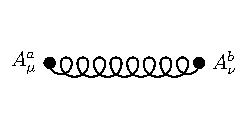
\includegraphics[width=.6\linewidth]{图/Ym-propa.pdf}
    \end{minipage} \begin{minipage}{.45\linewidth}
        \[i\Delta_{\mu\nu}^{ab} =\frac{-i\delta^{ab}}{k^2+i\epsilon}\left(\eta_{\mu\nu} - (1-\xi)\frac{k_\mu k_\nu}{k^2+i\epsilon} \right)\]
    \end{minipage}
    % \vspace{30pt}
\end{center}
\begin{center}
    \begin{minipage}{.5\linewidth}
\centering
%     \begin{fmffile}{YM-3vert}
%   \begin{fmfgraph*}(80,80)
%     \fmfleft{i1,i2}
%     \fmfright{i3}
%     \fmflabel{$A_\mu^a (p)$}{i1}
%     \fmflabel{$A_\nu^b (k)$}{i2}
%     \fmflabel{$A_\lambda^c (q)$}{i3}
%     \fmf{gluon}{i1,v,i2}
%     \fmf{gluon}{i3,v}
%   \end{fmfgraph*}
% \end{fmffile}
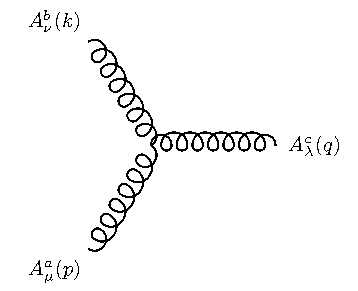
\includegraphics[width=.5\linewidth]{图/YM-3vert.pdf}
\end{minipage}\begin{minipage}{.5\linewidth}
        \[\Gamma_{\mu\nu\lambda}^{abc} = ig f^{abc}\Big( (p-k)_\lambda \eta_{\mu\nu} + (k-q)_\mu\eta_{\nu\lambda} + (q-p)_\nu\eta_{\mu\lambda} \Big)\]
    \end{minipage}
    % \vspace{30pt}
\end{center}
\begin{center}
    \begin{minipage}{.45\linewidth}
    \centering
%         \begin{fmffile}{Ym-4vert}
%   \begin{fmfgraph*}(70,70)
%     \fmfleft{i1,i2}
%     \fmfright{i3,i4}
%     \fmflabel{$A_\mu^a$}{i1}
%     \fmflabel{$A_\nu^b$}{i2}
%     \fmflabel{$A_\lambda^c$}{i3}
%     \fmflabel{$A_\rho^d$}{i4}
%     \fmf{gluon}{i1,v,i2}
%     \fmf{gluon}{i3,v,i4}
%   \end{fmfgraph*}
% \end{fmffile}
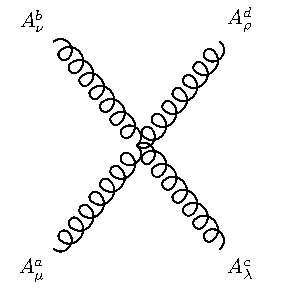
\includegraphics[width=.5\linewidth]{图/YM-4vert.pdf}
    \end{minipage}\begin{minipage}{.45\linewidth}
        \[\begin{split}
\Gamma^{abcd}_{\mu\nu\lambda\rho} = &-ig^2 \Big(f^{abe}f^{cde}(\eta_{\mu\lambda}\eta_{\nu\rho} - \eta_{\nu\lambda}\eta_{\mu\rho})\\ &+ f^{cbe}f^{ade}(\eta_{\mu\lambda}\eta_{\nu\rho}-\eta_{\mu\nu}\eta_{\lambda\rho})\\&+f^{dbe}f^{cae}(\eta_{\mu\nu}\eta_{\lambda\rho}-\eta_{\nu\lambda}\eta_{\mu\rho}) \Big)
        \end{split}\]
    \end{minipage}
        % \vspace{30pt}
\end{center}
\begin{center}
\centering
    \begin{minipage}{.45\linewidth}
    \centering
%         \begin{fmffile}{ghost-propa}
%   \begin{fmfgraph*}(120,20)
%     \fmfipair{i,o}
%     \fmfiequ{i}{(0.2w,0.5h)}
%     \fmfiequ{o}{(0.8w,0.5h)}
%     \fmfiv{d.sh=circle,d.f=1,d.si=2pt,l=$c^a$,l.a=180}{i}
%     \fmfiv{d.sh=circle,d.f=1,d.si=2pt,l=$c^b$,l.a=0}{o}
%     \fmfi{ghost,l.s=left}{i--o}
%   \end{fmfgraph*}
% \end{fmffile}
\vspace{10pt}
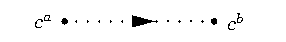
\includegraphics[width=.5\linewidth]{图/ghost-propa.pdf}
\vspace{10pt}
    \end{minipage} \begin{minipage}{.45\linewidth}
        \[i\Delta^{ab} =\frac{-i\delta^{ab}}{k^2+i\epsilon}\]
    \end{minipage}
    % \vspace{30pt}
\end{center}
\begin{center}
    \begin{minipage}{.45\linewidth}
\centering
%     \begin{fmffile}{ghost-YM-int}
%   \begin{fmfgraph*}(80,80)
%     \fmfleft{i1,i2}
%     \fmfright{i3}
%     \fmflabel{$c^a (p)$}{i1}
%     \fmflabel{$c^b (q)$}{i2}
%     \fmflabel{$A_\lambda^c (k)$}{i3}
%     \fmf{ghost}{i1,v,i2}
%     \fmf{gluon}{v,i3}
%   \end{fmfgraph*}
% \end{fmffile}
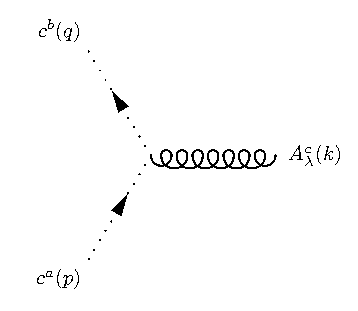
\includegraphics[width=.6\linewidth]{图/YM-ghost.pdf}
\end{minipage}\begin{minipage}{.45\linewidth}
        \[\Gamma_{\mu}^{abc} = -i\frac{g}{2} f^{abc} (k-p-q)_\mu \]
    \end{minipage}
    % \vspace{30pt}
\end{center}

\section{BRST(Becchi-Rouet-Stora-Tyutin)对称性}
现在考虑纯规范场的Lagrangian在洛伦兹规范下可表示为：
\begin{equation}
\mathscr{L}_\text{FP}=-\frac{1}{4}F^a_{\mu\nu}{F^a}^{\mu\nu}-\frac{\lambda}{2}(\partial^\mu A_\mu^a)^2+\partial^\mu\bar{c}^aD_\mu  c^a
\end{equation}
考虑对各场作如下变换：
\begin{equation}
\begin{split}
A^a_\mu&\rightarrow A^a_\mu+\epsilon D_\mu c^a\\
\bar{c}^a&\rightarrow\bar{c}^a-\epsilon \lambda\partial^\mu A_\mu^a\\
c^a&\rightarrow c^a+\epsilon 
\frac{g}{2} f^{abc} c^b c^c
\end{split}\label{eq:brsttrans}
\end{equation}
其中$\epsilon$为满足Grassmann代数的无穷小常量，和鬼场有反对易关系：
\begin{equation}
\{\epsilon,c\}=0,\qquad\{\epsilon,\bar{c}\}=0,\qquad[\epsilon,A_\mu^a]=0
\end{equation}
% 而$\tau$和$\rho$为待定常系数。
将变换带入Lagrangian，得到额外的项
\begin{equation}
    \delta\mathscr{L} = -\lambda\epsilon\partial^\mu D_\mu c^a\partial^\nu A^a_\nu -\lambda \epsilon\partial_\mu\partial^\nu A^a_\nu  D^\mu c^a + \frac{g}{2} \partial_\mu \bar{c}^a D^\mu( \epsilon f^{abc} c^b c^c)
\end{equation}
对第二项进行分部积分，可以将第一项抵消掉，得
\begin{equation}
    \delta\mathscr{L} =-\lambda\epsilon\partial_\mu(\partial^\nu A_\nu ^a D^\mu c^a) + \frac{g}{2} \partial_\mu \bar{c}^a D^\mu( \epsilon f^{abc} c^b c^c)
\end{equation}
对于最后一项，我们有
\begin{equation}
    \frac{g}{2}D^\mu( \epsilon f^{abc} c^b c^c) = -\frac{g^2}{2}(f^{acb}f^{bpq}-f^{apb}f^{bcq}-f^{aqb}f^{bpc})c^c c^p {A^\mu}^q \epsilon=0 
\end{equation}
因此Lagrangian只变化了一个全微分项
\begin{equation}
    \delta\mathscr{L} =-\lambda\epsilon\partial_\mu(\partial^\nu A_\nu ^a D^\mu c^a) = \epsilon\partial_\mu \Lambda^\mu,~~\Lambda^\mu = -\lambda\partial^\nu A^a_\nu D^\mu c^a\label{eq:brsttotd}
\end{equation}
则运动方程保持不变，则变换\eqref{eq:brsttrans}式即为BRST变换。

根据Nöther定理，我们可以通过下式计算守恒流
\begin{equation}
    J^\mu(\epsilon) = -\left( \frac{\partial \mathscr{L}_\text{FP}}{\partial(\partial_\mu A_\nu^a)}\delta A^a_\nu +\delta\bar{c}^a \frac{\partial \mathscr{L}_\text{FP}}{\partial(\partial_\mu\bar{c}^a)} + \frac{\partial \mathscr{L}_\text{FP}}{\partial (\partial_\mu c^a)}\delta c^a \right) + \epsilon \Lambda^\mu
\end{equation}
带入\eqref{eq:brsttrans}，\eqref{eq:brsttotd}式，可得
\begin{equation}
    J^\mu(\epsilon) =\epsilon J^\mu_\text{BRST} = \epsilon\left( -{F^{\mu\nu}}^aD_\nu c^a + \lambda\partial^\nu A_\nu^a D^\mu c^a + \frac{g}{2}f^{abc}\partial^\mu \bar{c}^a c^b c^c \right)
\end{equation}
最终我们可以得到BRST守恒荷
\begin{equation}
    Q_\text{BRST} = \int \mathrm{d}^3\boldsymbol{x} \left( -F^a_{0\nu}D^\nu c^a + \lambda\partial^\mu A_\mu ^a D_0 c^a + \frac{g}{2}f^{abc} \partial_0 \bar{c}^a c^b c^c\right)
    \end{equation}

    考虑我们存在杨-Mills场与Fermion场存在相互作用
    \begin{equation}
        \mathscr{L}=i\psi\slashed{D}\psi-m\bar{\psi}\psi-\frac{1}{4}F^a_{\mu\nu}{F^a}^{\mu\nu}-\frac{\lambda}{2}(\partial^\mu A_\mu^a)^2+\partial^\mu\bar{c}^aD_\mu  c^a
    \end{equation}
此时我们的BRST变换即为
\begin{equation}
\begin{split}
\delta A^a_\mu&= D_\mu c^a\\
\delta c^a&=-  \frac{g}{2} f^{abc} c^b c^c\\
\delta \bar{c}^a&=- \lambda\partial^\mu A_\mu^a\\
\delta \psi & = ig \,c^a \boldsymbol{T}^a \psi
\end{split}\label{eq:brsttrans_wf}
\end{equation}

\section{杨-Mills场单圈重整化}
对于杨-Mills场及参与规范相互作用的费米子场，其裸有效拉氏量为：
\begin{equation}
\begin{split}
    \mathscr{L}_0 = \bar{\psi}_0(i\slashed{\partial} - m_0-g_0 \slashed{A}^a_0\boldsymbol{T}^a)\psi_0 - \frac{1}{2}(\partial_\mu {A_0}_\nu^a \partial^\mu {{A_0}^a}^\nu-\partial_\mu {A_0}_\nu^a \partial^\nu {{A_0}^a}^\mu)-\frac{1}{2\xi_0}(\partial^\mu {A_0}_\mu^a)^2+\partial^\mu\bar{ c_0}^a\partial_\mu c_0^a \\
    -g'_0f^{abc} \partial_\mu {A_0}_\nu^a {{A_0}^\mu}^b{{A_0}^\nu}^c+\frac{1}{4}{g''_0}^2f^{abc}f^{ade}{A_0}_\mu^b {A_0}_\nu^c {{A_0}^\mu}^d {{A_0}^\nu}^e-g'''_0 f^{abc}(\partial^\mu\Bar{c_0}^a) c_0^b  {A_0}_\mu^c
\end{split}
\end{equation}
而重整化拉氏量即为拉氏量加上抵消项：
\begin{equation}
    \begin{split}
        \mathscr{L}_r =&(1+\delta_\psi)\bar{\psi}i\slashed{\partial}\psi  - m(1+\delta_m)\bar{\psi}\psi -(1+\delta_{g_1})g\mu^\epsilon \bar{\psi}\slashed{A}^a\boldsymbol{T}^a\psi - \frac{1+\delta_A}{2}(\partial_\mu {A}_\nu^a \partial^\mu {{A}^a}^\nu-\partial_\mu {A}_\nu^a \partial^\nu {{A}^a}^\mu)\\&-\frac{1+\delta_\xi}{2\xi}(\partial^\mu {A}_\mu^a)^2+(1+\delta_c)\partial^\mu\bar{ c}^a\partial_\mu c^a-g\mu^\epsilon(1+\delta_{g_2}) f^{abc} \partial_\mu {A}_\nu^a {{A}^\mu}^b{{A}^\nu}^c\\
        &+\frac{1+\delta_{g_3}}{4}{g}^2\mu^{2\epsilon}f^{abc}f^{ade}{A}_\mu^b {A}_\nu^c {{A}^\mu}^d {{A}^\nu}^e-g\mu^\epsilon(1+\delta_{g_4}) f^{abc}(\partial^\mu\Bar{c}^a) c^b  {A}_\mu^c
    \end{split}
\end{equation}
则我们有裸场与重整化场的关系：
\begin{equation}
    \psi_0 = \sqrt{1+\delta_\psi}\psi = \sqrt{Z_\psi}\psi,\quad{A_0}_\mu^a = \sqrt{1+\delta_A}A_\mu^a = \sqrt{Z_A}A_\mu^a,\quad c_0^a = \sqrt{1+\delta_c}c^a = \sqrt{Z_c}c^a
\end{equation}
对于裸耦合常数，裸质量及裸规范参数，我们则有：
\begin{align}
    m_0&= \frac{1+\delta_m}{1+\delta_\psi}m = \frac{Z_m}{Z_\psi}m\\
    g_0& = g\mu^\epsilon\frac{1+\delta_{g_1}}{(1+\delta_\psi)\sqrt{1+\delta_A}} = g\mu^\epsilon \frac{Z_1}{Z_\psi Z_A^{1/2}}\\
    g_0'& = g\mu^\epsilon \frac{1+\delta_{g_2}}{(1+\delta_A)^{3/2}}=g\mu^\epsilon\frac{Z_2}{Z_A^{3/2}}\\
    g_0''& = g\mu^\epsilon \frac{\sqrt{1+\delta_{g_3}}}{(1+\delta_A)^2} =g\mu^\epsilon\frac{Z_3^{1/2}}{Z_A^2}\\
    g_0'''&= g\mu^\epsilon \frac{1+\delta_{g_4}}{\sqrt{1+\delta_A}(1+\delta_c)}= g\mu^\epsilon\frac{Z_4}{Z_A^{1/2}Z_c}\\
    \xi_0& = \frac{1+\delta_A}{1+\delta_\xi}\xi=\frac{Z_A}{Z_\xi}\xi
\end{align}
此时，我们需要求解重整化参数$Z_\psi,~Z_A,~Z_c,~Z_m,~Z_\xi,~Z_{1-4}$，便可以对该理论进行重整化。而由于规范(BRST)对称性，这些裸耦合常数本为同一耦合常数$g_0=g'_0=g''_0=g'''_0$，因此有关系：
\begin{equation}
    Z_g= \frac{Z_1}{Z_\psi Z_A^{1/2}} = \frac{Z_2}{Z_A^{3/2}}=\frac{Z_3^{1/2}}{Z_A^{2}}=\frac{Z_4}{Z^{1/2}_AZ_c}
\end{equation}
此关系满足Slavnov–Taylor 恒等式，则我们并不需要求解所有的重整化参数，只需求解这6个独立的重整化参数$Z_\psi,~Z_A,~Z_c,~Z_m,~Z_\xi,~Z_{g}$。
\subsection{杨-Mills规范玻色子自能}
杨-Mills规范玻色子自能$\Pi^{ab}_{\mu\nu} =$包含了费米子圈，玻色子圈及鬼场圈的贡献：
\begin{center}
     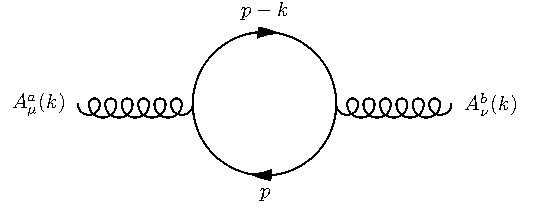
\includegraphics[width=.24\linewidth]{图/ymferloop.pdf}
% \begin{fmffile}{ymfermionloop}
%     \begin{fmfgraph*}(180,60)
%        \fmfleft{i}
%        \fmfright{o}
%        \fmfv{label=$A_\mu^a(k)$,l.a=180}{i}
%        \fmfv{label=$A_\nu^b(k)$,l.a=00}{o}
%        \fmf{gluon,tension=1}{i,v1} 
%        \fmf{gluon,tension=1}{v2,o}
%        \fmf{fermion,left,tension=0.4,label=$p$}{v2,v1}
%        \fmf{fermion,left,tension=0.4,label=$p-k$}{v1,v2}
%     \end{fmfgraph*}
% \end{fmffile}
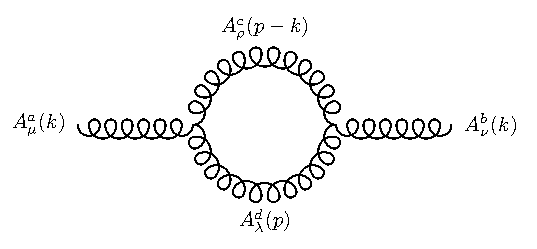
\includegraphics[width=.24\linewidth]{图/ymloop1.pdf}
% \begin{fmffile}{ymloop1}
%     \begin{fmfgraph*}(180,60)
%        \fmfleft{i}
%        \fmfright{o}
%        \fmfv{label=$A_\mu^a(k)$,l.a=180}{i}
%        \fmfv{label=$A_\nu^b(k)$,l.a=00}{o}
%        \fmf{gluon,tension=1}{i,v1} % ,label=H,label.side=left
%        \fmf{gluon,tension=1}{v2,o}
%        \fmf{gluon,left,tension=0.4,label=$A_{\lambda}^d(p)$}{v2,v1}
%        \fmf{gluon,left,tension=0.4,label=$A_{\rho}^c(p-k)$}{v1,v2}
%     \end{fmfgraph*}
% \end{fmffile}
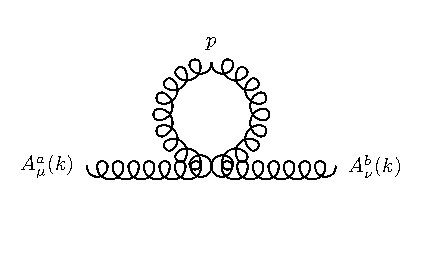
\includegraphics[width=.24\linewidth]{图/ymloop2.pdf}
% \begin{fmffile}{ymloop2}
% \begin{fmfgraph*}(120,100)
%        \fmfleft{i}
%        \fmfright{o}
%        \fmftop{m}
%        \fmfv{label=$A_\mu^a(k)$,l.a=180}{i}
%        \fmfv{label=$A_\nu^b(k)$,l.a=0}{o}
%        \fmflabel{$p$}{m}
%        \fmf{gluon,tension=1}{i,v1}
%        \fmf{gluon,tension=1}{v1,o}
%        \fmf{gluon,left,tension=0}{v1,m,v1}
%     \end{fmfgraph*}
% \end{fmffile}
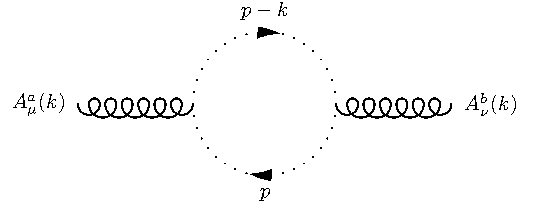
\includegraphics[width=.24\linewidth]{图/ymgholoop.pdf}
% \begin{fmffile}{ymghostloop}
%     \begin{fmfgraph*}(180,60)
%        \fmfleft{i}
%        \fmfright{o}
%        \fmfv{label=$A_\mu^a(k)$,l.a=180}{i}
%        \fmfv{label=$A_\nu^b(k)$,l.a=00}{o}
%        \fmf{gluon,tension=1}{i,v1} % ,label=H,label.side=left
%        \fmf{gluon,tension=1}{v2,o}
%        \fmf{ghost,left,tension=0.4,label=$p$}{v2,v1}
%        \fmf{ghost,left,tension=0.4,label=$p-k$}{v1,v2}
%     \end{fmfgraph*}
% \end{fmffile}
\end{center}
\paragraph{费米子圈}

根据费曼圈积分公示，规范玻色子的费米子圈图即为圈积分：

\begin{figure}[h]
    \centering
    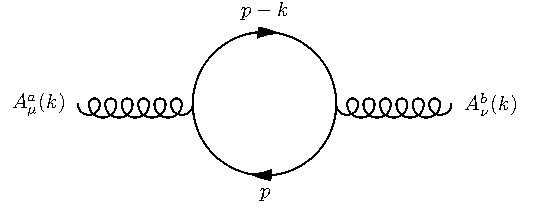
\includegraphics[width=.38\linewidth]{图/ymferloop.pdf}
    \caption{}
    \label{fig:ymferloop}
\end{figure}
\begin{equation}
\begin{split}
\Pi^{ab}_{\mu\nu}(k)&=-\int\frac{\mathrm{d}^{4-\epsilon} p}{(2\pi)^{4-\epsilon}}\operatorname{Tr}\Big[(-ig_0\boldsymbol{T}^a\gamma_\mu)\frac{ i}{\slashed{p}-m}(-ig_0\boldsymbol{T}^b\gamma_\nu)\frac{ i}{\slashed{p}-\slashed{k}-m}\Big]    \\
&=\frac{-i8g^2\mu^{2\epsilon}}{16\pi^2}\operatorname{Tr}(\boldsymbol{T}^a\boldsymbol{T}^b)(k_\mu k_\nu-\eta_{\mu\nu}k^2)\Gamma(\frac{\epsilon}{2})\int_0^1\mathrm{d}x\left(\frac{k^2 x(1-x)+m^2}{4\pi}\right)^{-\frac{\epsilon}{2}}\Big[(x-1)x\Big]
\end{split}
\end{equation}
可以求得：
\begin{equation}
   \Pi^{ab}_{\mu\nu}(k) = \frac{ig^2\delta^{ab}}{16\pi^2}(\eta_{\mu\nu}k^2 - k_\mu k_\nu)\Big[ -\frac{4}{3\epsilon} + 8\int_0^1 (1-x)x\ln\frac{k^2 x(1-x)+m^2}{\mu^2} +\text{finite.}\Big] 
   \label{eq:ymferloop}
\end{equation}


\section{规范对称性自发破缺与BEH机制}
对于杨-Mills场而言，场的质量项$mA_\mu A^\mu$显然破坏了规范对称性，因此杨-Mills场必须为无质量场。然而当我试图描述带质量的规范相互作用时，我们则需要引入额外的机制赋予规范场的质量项。这样的机制假定规范对称性存在于在高能标的情形，此时规范场不具有质量。而当系统自然地过渡到低能标时，规范场的质量项自发的产生，则规范对称性同时自发地被破坏，即称之为“规范对称性自发破缺”。

通常来说场的基态即为真空态，其真空期望值通常为零。然而我们假设拉格朗日中存在某个场，其真空期待值为非零值，那么该场的自由度将会在高于其它场基态的能标中冻结。如果该场还具有不同分量，其分量之间存在着规范对称性，那么如果该场不同分量之间的规范对称性在基态中被破坏的话，便可以在其它场仍能处于自由态的时候，自发的破坏规范对称性。

% 显性的对称性破缺意味着Lagrangian中存在某项，其在对称性变换下无法保持不变。而自发的对称性破缺则是Lagrangian在对称性变换下通常保持不变，但是当系统处于基态时，真空却不是唯一的。如果系统的真空态只有一个，则为对称群中的单态，那么自发对称性破缺则不会发生。而如果真空存在多个简并态，则这些真空态为对称群中的非单态，那么当系统能量最低时，必然只会成为一个物理真空态，此时该物理真空态相对于群中其它的简并真空态而言就是独特的，对称性因此而破缺。

% 我们在研究自然界的基本原理时，往往需要借助对称性来描述一类事物具有的共性。这样的理论虽然十分成功，但是在实际情况中，事物却并不总是表现为具有普遍的共性，而是往往表现为具有普遍的差异性。这就意味着，对称性的破缺现象才是在自然界中普遍存在的。



% 我们以标量场为例：
% \begin{equation}
%     \mathscr{L}=\frac{1}{2}\partial_\mu\phi\partial^\mu\phi-\frac{1}{2}\mu^2\phi^2-\frac{\lambda}{4}\phi^4
% \end{equation}
% 其中场具有内禀对称性$\phi\rightarrow e^{i\alpha}\phi$。此时Lagrangian中的标量势为$V=\frac{1}{2}\mu^2\phi^2+\frac{\lambda}{4}\phi^4$，那么对标量势求一阶导可以找出势能的极小值点，也即真空态：
% \begin{equation}
%     \frac{\partial V}{\partial\phi}=\mu^2\phi+\lambda\phi^3=0
% \end{equation}
% \begin{figure}[H]
%     \centering
% \begin{minipage}{.4\textwidth}
%     \centering
%     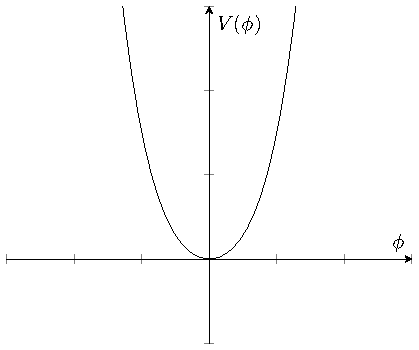
\includegraphics[width=\textwidth]{图/fig_pot_2.pdf}
%     \caption*{$\mu^2>0$}
% \end{minipage}\hfill
% \begin{minipage}{.4\textwidth}
%     \centering
% 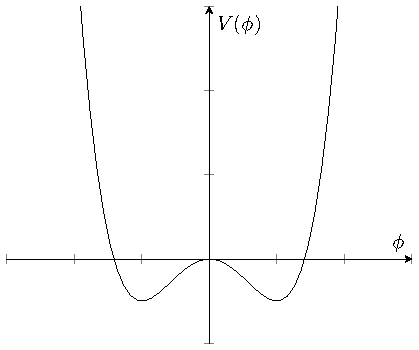
\includegraphics[width=\textwidth]{图/fig_pot_1.pdf}
%  \caption*{$\mu^2<0$}
% \end{minipage}
% \caption{}
% \end{figure}
% 此时当$\mu^2>0$时，标量场$\phi$有且只有一个实根，即标量场的真空期望值$\langle0|\phi|0\rangle=0$，那么真空态即为单态，不发生对称性自发破缺。\\
% 而当$\mu^2<0$时，标量场$\phi$则有非零实根：
% \begin{equation}
%     \langle0|\phi|0\rangle=v=\pm\sqrt{\frac{-\mu^2}{\lambda}}
% \end{equation}
% 此时存在两个简并的真空态，即对应真空期望值$v$为正或负的两个态，但是实际只能有一个物理的真空态。当我们考虑内禀对称性时，可以取参数$\alpha=\pi$，那么对称变换即为$\phi\rightarrow-\phi$，那我们将此对称性带入到真空态时，可得：
% \begin{equation}
%     v=\langle0|\phi|0\rangle\rightarrow \langle0|-\phi|0\rangle=-v
% \end{equation}
% 显然，只要当$v\neq0$时，该对称性在真空态中就不再成立。

% 考虑对称性自发破缺的情况，那么我们定义新的场函数：
% \begin{equation}
%     \phi\rightarrow v+\phi
% \end{equation}
% 带入回Lagrangian中便可得真空态的情形：
% \begin{align}
%     \mathscr{L}&=\frac{1}{2}\partial_\mu\phi\partial^\mu\phi-(\mu^2+\lambda v^2)v\phi-\frac{{\mu^2}+3\lambda v^2}{2}\phi^2-\lambda v\phi^3-\frac{\lambda}{4}\phi^4-\frac{v^2}{2}(\mu^2+\frac{\lambda v^2}{2})\notag\\
%     &=\frac{1}{2}\partial_\mu\phi\partial^\mu\phi-\lambda v^2\phi^2-\lambda v\phi^3-\frac{\lambda}{4}\phi^4+\frac{\lambda}{4}v^4
% \end{align}
% 其中利用了$\mu^2=-\lambda v^2$。此时标量子的质量则为$m=\sqrt{2\lambda}v$，且获得了额外的三相互作用顶点。
我们现在考虑一个复标量场$\phi$，该场具有自相互作用势能$V(\phi)$:
\begin{gather}
    \mathscr{L}=\partial^\mu\phi^\dagger\partial_\mu\phi-V(\phi)\\
    V(\phi)=\mu^2\phi^\dagger\phi+{\lambda}(\phi^\dagger\phi)^2
\end{gather}
同时该场具有SU($N$)规范对称性$\phi(x)\rightarrow e^{i\omega^a(x)\boldsymbol{T}^a}\phi(x)$，其分量为SU($N$)规范对称群的多重态。那么在场处于真空态时，有势能极小值条件：
\begin{equation}
    \frac{\partial V}{\partial\phi}=\Big(\mu^2+2\lambda(\phi^\dagger\phi)\Big)\phi^\dagger=0
\end{equation}
\begin{figure}[h]
    \centering
    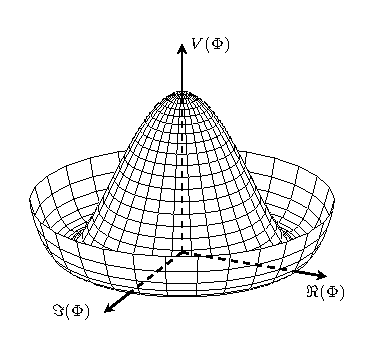
\includegraphics{图/higgspot.pdf}
    \caption{}
    \label{fig:higgspot}
\end{figure}
当$\mu^2>0$时，只有唯一真空态，其真空期望值为$\langle0|\phi|0\rangle=0$。而当$\mu^2<0$时，势能的形状则如图\ref{fig:higgspot}所示，存在非平庸真空期待值：
\begin{equation}
    \langle0|\phi^\dagger\phi|0\rangle=-{\frac{\mu^2}{2\lambda}}=\frac{v^2}{2}
\end{equation}
由于$\phi$为规范群多重态，所以$|\phi|^2=\sum^N_i \phi_i^*\phi_i=\sum^N_i(\Re(\phi_i)^2+\Im(\phi_i)^2)=\frac{v^2}{2}$。此时我们有无限多个简并的真空态，那么我们人为选定其中一个分量$\langle0|\Re(\phi_i)|0\rangle=v/\sqrt{2}$，其它所有分量的真空期待值为0，即：
\begin{equation}
    \langle0|\phi|0\rangle=\begin{pmatrix}
    0\\
    \vdots\\
    \frac{v}{\sqrt{2}}%\\
    %0&  \cdots& v
    \end{pmatrix}
\end{equation}
我们对场的真空态作对称变换：
\begin{align}
    \frac{v_i}{\sqrt{2}}=\langle0|\phi_i|0\rangle\rightarrow&\langle0|e^{i\omega^a\boldsymbol{T}^a}\phi_i|0\rangle=\langle0|(1+{i\omega^a\boldsymbol{T}^a_{ij}})\phi_i|0\rangle\notag\\
    &=\frac{v_i}{\sqrt{2}}+i\omega^a\langle0|\boldsymbol{T}^a_{ij}\phi_i|0\rangle
\end{align}
如果真空态在规范变换下不变，那么我们显然可得只有当$\langle0|\boldsymbol{T}_{ij}^a\phi_i|0\rangle=0$时，规范对称性在真空态中才能保存。然而这条件并不能对所有群生产元$\boldsymbol{T}^a$成立。因此由于非零真空期待值的存在，这些简并态之间本来存在的SU($N$)规范对称性便遭到破坏，即为规范对称性的自发破缺。

然而对于$\langle0|\boldsymbol{T}_{ij}^a\phi_i|0\rangle=0$的情况，实际上意味着在规范群$G$中，存在着不变子群$H\subset G$，使得即使在真空态中规范对称性被破坏时，该子群的元素依然保留着规范对称性。对于这种特殊情况，我们考虑真空态中的势$V(\phi)$，其具有规范对称性：
\begin{equation}
    \langle0|\delta V|0\rangle=\langle0|\frac{\partial V}{\partial \phi_i}\delta\phi_i|0\rangle = i\omega^a \langle0|\frac{\partial V}{\partial \phi_i}\boldsymbol{T}^a_{ij} \phi_j|0\rangle=0
\end{equation}
由于$\omega^a$为任意参数，因此有：
\begin{equation}
    \langle0|\frac{\partial V}{\partial \phi_i}\boldsymbol{T}^a_{ij} \phi_j|0\rangle=0
\end{equation}
然后在对此作一次微商：
\begin{equation}
       \frac{\partial^2 V}{\partial \phi_i\partial\phi_k}\Big|_{\phi = v/\sqrt{2}}\langle0|\boldsymbol{T}^a_{ij} \phi_j|0\rangle+\frac{\partial V}{\partial \phi_i} \Big|_{\phi = v/\sqrt{2}}\boldsymbol{T}^a_{ik}=0
\end{equation}
其中由于$\phi = v/\sqrt{2}$处为势的极小值点，所以有$\frac{\partial V}{\partial \phi_i} \Big|_{\phi = v/\sqrt{2}}=0$，则可得：
\begin{equation}
    \frac{\partial^2 V}{\partial \phi_i\partial\phi_k}\Big|_{\phi = v/\sqrt{2}}\langle0|\boldsymbol{T}^a_{ij} \phi_j|0\rangle=0
    \label{eq:gsth}
\end{equation}
如果我们将势围绕真空态展开，则有：
\begin{equation}
    V(\phi)=V(v) +\frac{1}{2}\frac{\partial^2 V}{\partial \phi_i\partial\phi_k}\Big|_{\phi = v/\sqrt{2}}(\phi_i-\frac{v}{\sqrt{2}})(\phi_k-\frac{v}{\sqrt{2}})+\cdots
\end{equation}
而势的二阶微商则为场的质量项，因此我们可以得到场的质量矩阵：
\begin{equation}
    M^2_{ij}=\frac{\partial^2 V}{\partial \phi_i\partial\phi_k}\Big|_{\phi = v/\sqrt{2}}
\end{equation}
从\eqref{eq:gsth}式中，我们容易看出，当$\langle0|\boldsymbol{T}^a_{ij} \phi_j|0\rangle\neq0$时，必然有$M^2_{ik}=0$。而当$\langle0|\boldsymbol{T}^a_{ij} \phi_j|0\rangle=0$时，则有可能存在非零质量项。综合之前的讨论，对于规范群$G$中的子群$H$以外的部分，其维度为$\mathrm{dim}(G/H)=\mathrm{dim}(G)-\mathrm{dim}(H)$，则总体系中至少存在$\mathrm{dim}(G/H)$个无质量标量场，我们称此场为Goldstone玻色子。%，该结论即为Goldstone定理。
因此，我们可得Goldstone定理：当一个自由度为$n$的连续对称型自发破缺之后，必然会产生$n$个Goldstone玻色子。

现在我们可以在围绕真空期望值的基础上定义无穷小的新场：
\begin{equation}
    \phi(x)=\frac{v+ H(x)}{\sqrt{2}}\exp\left(i\frac{\omega^a(x)\boldsymbol{T}^a}{v}\right)
    \label{eq:phiv}
\end{equation}
其中$H(x)$为实标量场，带入回Lagrangian中，得：
\begin{align}
    \mathscr{L}=&\frac{1}{2}\partial^\mu H\partial_\mu H+\frac{1}{2}\left(1+\frac{H}{v}\right)^2\partial^\mu\omega^a\partial_\mu\omega^a-\frac{1}{2}\mu^2(v+ H)^2-\frac{\lambda}{4}(v+ H)^4%\notag\\
    % \approx&\partial^\mu\rho\partial_\mu\rho+v^2\partial^\mu\omega^a\partial_\mu\omega^a-2\lambda v^2\rho^2-2\lambda v\rho^3-\frac{\lambda}{2}\rho^4+\cdots\notag\\
    % \approx&\partial^\mu\rho\partial_\mu\rho+v^2\partial^\mu\omega^a\partial_\mu\omega^a-2\lambda v^2\rho^2+\text{interactions}
\end{align}
同时将$\lambda=-\mu^2/v^2$带入，得
\begin{equation}
\begin{split}
    \mathscr{L}=&\frac{1}{2}\partial^\mu H\partial_\mu H+\mu^2 H^2  +\frac{\mu^2}{v} H^3+\frac{\mu^2}{4v^2} H^4+\frac{1}{2}\mu^2 v^2\\
    &+ \frac{1}{2} \partial^\mu\omega^a\partial_\mu\omega^a +\frac{H}{v} \partial^\mu\omega^a\partial_\mu\omega^a + \frac{H^2}{2v^2}\partial^\mu\omega^a\partial_\mu\omega^a
\end{split}
\end{equation}
可以看到，只有$ H$场获得了质量$m^2=-2\mu^2$，而所有其它的$\omega^a$场都为无质量的玻色子场。我们可得：
\begin{equation}
\begin{split}
    \mathscr{L}=&\frac{1}{2}\partial^\mu H\partial_\mu H-\frac{1}{2}m^2 H^2  -\frac{m^2}{2v} H^3-\frac{m^2}{8v^2} H^4-\frac{1}{4}m^2 v^2\\
    &+ \frac{1}{2} \partial^\mu\omega^a\partial_\mu\omega^a +\frac{H}{v} \partial^\mu\omega^a\partial_\mu\omega^a + \frac{1}{2v^2}H^2\partial^\mu\omega^a\partial_\mu\omega^a
\end{split}
\end{equation}

当我们考虑该场参与规范相互作用时，则有：
\begin{equation}
    \mathscr{L}=(D^\mu\phi)^\dagger D_\mu\phi-V(\phi),\qquad D_\mu = \partial_\mu -igQ A_\mu%^a \boldsymbol{T}^a
\end{equation}
我们得：
\begin{equation}
    \mathscr{L}=\partial^\mu\phi^\dagger\partial_\mu\phi+g^2Q^2A_\mu A^\mu \phi^\dagger\phi + igQA_\mu(\phi^\dagger\partial^\mu \phi - \partial^\mu\phi^\dagger \phi)-V(\phi)
\end{equation}
同理，我们带入真空态附近的场函数\eqref{eq:phiv}，我们可得：
\begin{equation}
\begin{split}
    \mathscr{L}=&\frac{1}{2}\partial^\mu H\partial_\mu H-\frac{1}{2}m^2 H^2  -\frac{m^2}{2v} H^3-\frac{m^2}{8v^2} H^4-\frac{1}{4}m^2 v^2\\
    &+  \frac{g^2Q^2v^2}{2}A_\mu A^\mu + g^2Q^2 v A_\mu A^\mu  H + \frac{g^2Q^2}{2}  H^2 A_\mu A^\mu\\
    &+ \left(1+\frac{H}{v}\right)^2\frac{1}{2}\partial^\mu\omega \partial_\mu\omega  -g v A_\mu \partial^\mu\omega \left(1+\frac{H}{v}\right)^2
\end{split}
\end{equation}
则规范场$A_\mu$获得了质量项$m_A^2=g^2 Q^2 v^2$，Lagrangian可以写为：
\begin{equation}
\begin{split}
    \mathscr{L}=&\frac{1}{2}\partial^\mu H\partial_\mu H-\frac{1}{2}m^2 H^2  -\frac{m^2}{2v} H^3-\frac{m^2}{8v^2} H^4-\frac{1}{4}m^2 v^2\\
    &+ \frac{1}{2}\partial^\mu\omega \partial_\mu\omega  +\frac{H}{v} \partial^\mu\omega \partial_\mu\omega  + \frac{1}{2v^2}H^2\partial^\mu\omega \partial_\mu\omega \\
    &+ \frac{1}{2}m_A^2 A_\mu A^\mu + \frac{m_A^2}{v} A_\mu A^\mu  H +\frac{m_A^2}{2v^2} H^2 A_\mu A^\mu\\
    &-m_A A_\mu \partial^\mu\omega - 2\frac{m_A}{v} H A_\mu\partial^\mu\omega - \frac{m_A}{v^2} H^2 A_\mu\partial^\mu\omega
\end{split}
\end{equation}
其中$-m_A A_\mu \partial^\mu\omega$项会带来$A_\mu$场和$\omega$场的混合，而由于$A_\mu$场的规范对称性，我们可以引入一个规范场的规范变换来消除掉该项，称之为幺正规范。此时新的规范场为：
\begin{equation}
    A_\mu \rightarrow e^{\frac{-i\omega(x)}{v}}A_\mu e^{\frac{i\omega(x)}{v}} - \frac{1}{m_A}\partial_\mu \omega(x)
\end{equation}
此时，我们可得：
\begin{equation}
    D_\mu \phi = \frac{1}{\sqrt{2}}e^{\frac{-i\omega(x)}{v}}(\partial_\mu H -igA'_\mu (v+H))
\end{equation}
则Lagrangian为：
\begin{equation}
\begin{split}
    \mathscr{L}=&\frac{1}{2}\partial^\mu H\partial_\mu H-\frac{1}{2}m^2 H^2  -\frac{m^2}{2v} H^3-\frac{m^2}{8v^2} H^4-\frac{1}{4}m^2 v^2\\
    &+ \frac{1}{2}m_A^2 A_\mu {A}^\mu + \frac{m_A^2}{v} A_\mu {A}^\mu  H +\frac{m_A^2}{2v^2} H^2 A_\mu {A}^\mu
\end{split}
\end{equation}

因此，我们可以看出，规范场$A_\mu$通过这样的规范对称性破缺机制获得了质量项，并同时将无质量的Goldestone玻色子场$\omega$“吃掉”，这样的机制即为Brout-Englert-Higgs机制，而标量场$\phi$即为Higgs场，产生的标量粒子即为Higgs玻色子。
% \section{基本粒子标准模型}

% 标准粒子物理模型包含了组成物质的费米子以及传递相互作用的规范玻色子，其中胶子作为SU(3)$_\text{C}$规范群的生成元传递了夸克间的强相互作用，而$W/Z$玻色子作为SU(2)$_\text{L}$群生成元传递弱相互作用。
而对于规范群中的费米子而言，我们考虑中其与Higgs场的相互作用：%在Weyl表象
\begin{equation}
    \mathscr{L}=i\bar{\psi}\slashed{D}\psi  - (Y_\text{f} \bar{\psi}_L \phi \psi_R+\mathrm{h.c.}) - V(\phi)
    \label{eq:Higgsfermions}
\end{equation}
其中$Y_f$称之为汤川耦合，即为汤川相互作用。当费米子和Higgs场都为规范SU(2)群的多重态时，Higgs场具有4个分量，因此Higgs势$V(\phi)$具有整体SO(4)对称性。由于SO(4)对称性同构于两个独立的SU(2)对称性，因此方程\eqref{eq:Higgsfermions}中的Lagrangian具有整体的SO(4)$=$SU($N)_L\otimes$SU($N)_R$对称性，即Lagrangian在以下变换中
\begin{gather}
    \phi\rightarrow e^{i\alpha_L^a\boldsymbol{T}^a }\phi~ e^{-i\alpha_R^a\boldsymbol{T}^a }\\
    \psi_L \rightarrow e^{i\alpha_L^a\boldsymbol{T}^a }\psi_L\\
    \psi_R \rightarrow e^{i\alpha_R^a\boldsymbol{T}^a }\psi_R
\end{gather}
保持不变。其中在Weyl表象中分别对应了左手费米子$\psi_L$的整体SU(2)$_L$对称性和右手费米子$\psi_R$的整体SU(2)$_R$对称性。
但是当规范对称性破缺时，该整体对称性也会发生破缺，此时Higgs势的整体对称性破缺为SO(3)对称性，同构于SU(2)对称性。在Weyl表象中则表为
\begin{equation}
    \mathrm{SU(2)}_L\otimes\mathrm{SU(2)}_R\rightarrow \mathrm{SU(2)}_V
\end{equation}
即费米子在发生规范对称性自发破缺以后，依然保留了SU(2)$_V$对称性，称之为看守对称性。

总而言之，我们可以将规范群中的费米子场和Higgs场，以及规范玻色子场综合起来，得到如下Lagrangian：
\begin{equation}
    \mathscr{L}=(D^\mu \phi)^\dagger (D_\mu \phi) + i\bar{\psi}\slashed{D}\,\psi -\frac{1}{4}{F^a}_{\mu\nu}{F^a}^{\mu\nu}  - (Y_\text{f} \,\bar{\psi}_L \phi\, \psi_R+\mathrm{h.c.}) - V(\phi)
    \label{eq:smlagrangian}
\end{equation}
即为粒子物理标准模型Lagrangian。
